\documentclass{dissertation}

\begin{document}

%% Specify the title and author of the thesis. This information will be used on
%% the title page (in title/title.tex) and in the metadata of the final PDF.
\title[Optional Subtitle]{Title}
\author{Albert}{Einstein}

%% Use Roman numerals for the page numbers of the title pages and table of
%% contents.
\frontmatter

\begin{titlepage}

\begin{center}

%% Extra whitespace at the top.
\vspace*{2\bigskipamount}

%% Print the title.
{\makeatletter
\titlestyle\singlespacing\bfseries\LARGE\@title\par
\makeatother}

%% Print the optional subtitle.
{\makeatletter
\ifx\@subtitle\undefined\else
    \bigskip
    \titlefont\titleshape\Large\@subtitle
\fi
\makeatother}

\end{center}

\cleardoublepage
\thispagestyle{empty}

\begin{center}

%% The following lines repeat the previous page exactly.

\vspace*{2\bigskipamount}

%% Print the title.
{\makeatletter
\titlestyle\singlespacing\bfseries\LARGE\@title\par
\makeatother}

%% Print the optional subtitle.
{\makeatletter
\ifx\@subtitle\undefined\else
    \bigskip
    \titlefont\titleshape\Large\@subtitle
\fi
\makeatother}


%% Uncomment the following lines to insert a vertically centered picture into
%% the title page.
%\vfill
%\includegraphics{title}
\vfill

%% Apart from the names and dates, the following text is dictated by the
%% promotieregelement.

{\Large\titlefont\bfseries Proefschrift}

\bigskip
\bigskip

ter verkrijging van de graad van doctor

aan de Technische Universiteit Delft,

op gezag van de Rector Magnificus prof.~???,

voorzitter van het College voor Promoties,

in het openbaar te verdedigen op dinsdag 1 Maart 2023 om 10:00 uur

\bigskip
\bigskip

door

\bigskip
\bigskip

%% Print the full name of the author.
\makeatletter
{\Large\titlefont\bfseries\@firstname\ {\titleshape\@lastname}}
\makeatother
\\
\vspace{3mm}
\begin{CJK*}{UTF8}{gkai}
\makeatletter
{\LARGE\titlefont\bfseries\@lastnameCH\ \hspace{1mm} {\titleshape\@firstnameCH}}
\makeatother
\end{CJK*}

\bigskip
\bigskip

Master of Science in Applied Physics,

Delft University of Technology, the Netherlands,

geboren te Hohhot, P.~R.~China.

%% Extra whitespace at the bottom.
\vspace*{2\bigskipamount}

\end{center}

\clearpage
\thispagestyle{empty}

%% The following line is dictated by the promotieregelement.
\noindent Dit proefschrift is goedgekeurd door de promotor:

%% List the promotors (supervisors).
\medskip\noindent
\begin{tabular}{l}
    Prof.\ dr.\ H.\ P.\ Urbach
\end{tabular}

%% List the (optional) copromotor.
\medskip
\noindent Copromotor: Dr.\ F.\ Bociort

\medskip
\noindent Samenstelling promotiecommissie:

%% List the committee members, starting with the Rector Magnificus and the
%% promotor(s) and ending with the reserve members.
\medskip\noindent
\begin{tabular}{ll}
    Rector Magnificus, & voorzitter \\
    Prof.\ dr.\ H.\ P.\ Urbach, & Technische Universiteit Delft, promotor \\
    Dr.\ F.\ Bociort, & Technische Universiteit Delft, copromotor \\
    ??? & ??? \\
    ??? & ??? \\
    ??? & ??? \\
    ??? & ??? \\
    ??? & ??? \\
\end{tabular}

%% Include the following disclaimer for committee members who have contributed
%% to this dissertation. Its formulation is again dictated by the
%% promotieregelement.
\medskip
\noindent Prof.\ dr.\ ir.\ ???.\ ??? heeft als begeleider in belangrijke mate aan de totstandkoming van het proefschrift bijgedragen.

%% Here you can include the logos of any institute that contributed financially
%% to this dissertation.
\vfill
\begin{center}
    
\includegraphics[height=0.6in]{title/logos/tudelftpng}
    \hspace{2em}
    
\includegraphics[height=0.6in]{title/logos/marie-curie}
    \hspace{2em}
    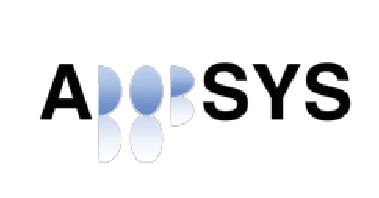
\includegraphics[height=0.55in]{title/logos/adopsys}
\end{center}
\vfill

\noindent
\begin{tabular}{@{}p{0.2\textwidth}@{}p{0.8\textwidth}}
    \textit{Keywords:} & \ldots \\[\medskipamount]
    \textit{Printed by:} & Johannes Gutenberg \\[\medskipamount]
    \textit{Front \& Back:} & Beautiful cover art that captures the entire content of this thesis in a single illustration.
\end{tabular}

\vspace{4\bigskipamount}

\noindent Copyright \textcopyright\ 2022 by Zhe Hou

%% Uncomment the following lines if this dissertation is part of the Casimir PhD
%% Series, or a similar research school.
%\medskip
%\noindent Casimir PhD Series, Delft-Leiden 2013-01

\medskip
\noindent ISBN 000-00-0000-000-0

\medskip
\noindent An electronic version of this dissertation is available at \\
\url{http://repository.tudelft.nl/}.

\newpage
\;
\vspace{12em}



% Here is the explanation about the cover
\begin{figure}[h!]
    \centering
    
\includegraphics[scale=0.35]{cover/CoverSP.png}
\end{figure} 
Designed by Hui Lin

 The concept is borrowed from Escher's style. We draw horse patterns together with the "saddle" which relates to the "saddle point". In between the horse patterns, there are pieces of convex and concave lens shape. I would like to indicate a lens design network or space that the lens solutions are linked/surrounded by saddles (saddle points). In a whole, with Escher's way of presenting, the pattern seems quite complicated, yet is composed with a monotonic repetitive pattern (the feeling of the complexity is probably from the color composition and angular arrangement). It is sort of related to the goal of the thesis/research: in a complicated design landscape, we are trying to find a systematic way to describe it and then utilize knowledge for practical design. 

\end{titlepage}



%% The (optional) dedication can be used to thank someone or display a
%% significant quotation.
\dedication{\epigraph{Science is a wonderful thing \\ if one does not have to earn one's living at it.}{Albert Einstein}}

\chapter*{Preface}
\setheader{Preface}

Preface\ldots

\begin{flushright}
\LARGE\textbf{unnecessary}
{\makeatletter\itshape
    \@firstname\ \@lastname \\
    Delft, January 2013
\makeatother}
\end{flushright}



\tableofcontents

%% Use Arabic numerals for the page numbers of the chapters.
\mainmatter

%% Turn on thumb indices.
\thumbtrue

\chapter{Introduction}
\label{chapter_1}

%% The following annotation is customary for chapter which have already been
%% published as a paper.
\blfootnote{Parts of this chapter have been published in Annalen der Physik \textbf{324}, 289 (1906) \cite{Einstein1906}.}

%% It is only necessary to list the authors if multiple people contributed
%% significantly to the chapter.
\authors{Albert {\titleshape Einstein}}

%% The '0pt' option ensures that no extra vertical space follows this epigraph,
%% since there is another epigraph after it.
\epigraph[0pt]{
    Nature and nature's laws lay hid in the night; \\
    God said `Let Newton be!' and all was light.
}{Alexander Pope}

\epigraph{
    It did not last: the devil shouting `Ho. \\
    Let Einstein be!' restore the status quo.
}{Sir John Collings Squire}

\begin{abstract}
Lorem ipsum dolor sit amet, consectetur adipisicing elit, sed do eiusmod tempor incididunt ut labore et dolore magna aliqua. Ut enim ad minim veniam, quis nostrud exercitation ullamco laboris nisi ut aliquip ex ea commodo consequat. Duis aute irure dolor in reprehenderit in voluptate velit esse cillum dolore eu fugiat nulla pariatur. Excepteur sint occaecat cupidatat non proident, sunt in culpa qui officia deserunt mollit anim id est laborum.
\end{abstract}

%% Start the actual chapter on a new page.
\newpage

\noindent This document is intended to be both an example of the TU Delft dissertation template for \LaTeX, as well as a short introduction to its use. It is not intended to be a general introduction to \LaTeX{} itself,\footnote{We recommend \url{http://en.wikibooks.org/wiki/LaTeX} as a reference and a starting point for new users.} and we will assume the reader to be familiar with the basics of creating and compiling documents.

Instructions on how to use this template under Windows and Linux, and which \LaTeX{} packages are required, can be found in \texttt{README.txt}.

%%%%%%%%%%%%%%%%%%%%%%%%%% SECTION 1 %%%%%%%%%%%%%%%%%%%%%%%%%%%%%%%%%%%%%%%%%%%%%%%%%%%%%%%%
\section{Problem for optical system design}
\vspace{1em}
How does this nonlinearty appear?

%% We need an empty line before the quote environment to work around a bug in
%% the lettrine package, from which the drop command is derived.
\begin{quote}
\texttt{\textbackslash documentclass\{dissertation\}}
\end{quote}
which loads the dissertation template. The template is based on the \LaTeX{} \texttt{book} document class and stored in \texttt{dissertation.cls}. The document class accepts several comma-separated options. By default, hyperlinks are shown in cyan, which is convenient when reading the dissertation on a computer, but can be expensive when printing. They can be turned black with the \texttt{print} option. This will also turn the headers dark gray instead of cyan. Moreover, it will add a 3~mm bleed around the page including crop marks. This will help the printer with the thumb indices, since they run right up to the page borders. Finally, the \texttt{nativefonts} option can be used to override the automatic font selection (see below).

A dissertation is a big document, which makes it easy to miss warnings about the layout in the \LaTeX{} output. In order to locate problem areas, add the \texttt{draft} option to the \texttt{\textbackslash documentclass} line. This will display a vertical bar in the margins next to the paragraphs that require attention.

The contents of the dissertation are included between the \texttt{\textbackslash begin\{document\}} and \texttt{\textbackslash end\{document\}} commands, and split into three parts by
\begin{enumerate}
\item\texttt{\textbackslash frontmatter}, which uses Roman numerals for the page numbers and is used for the title page and the table of contents;
\item\texttt{\textbackslash mainmatter}, which uses Arabic numerals for the page numbers and is the style for the chapters;
\item\texttt{\textbackslash appendix}, which uses letters for the chapter numbers, starting with `A'.
\end{enumerate}
The title page is defined in \texttt{title.tex} in the \texttt{title} folder and included verbatim with \texttt{\textbackslash include\{title/title\}},\footnote{Note that it is not necessary to specify the file extension.} (see below). Additionally, it is possible to include a preface, containing, for example, the acknowledgements. An example can be found in \texttt{preface.tex}. The table of contents is generated automatically with the \texttt{\textbackslash tableofcontents} command. Chapters are included after \texttt{\textbackslash mainmatter} and appendices after \texttt{\textbackslash appendix}. For example, \texttt{\textbackslash include\{chapter-1/chapter-1\}} includes \texttt{chapter-1.tex}, which contains this introduction.

%%%%%%%%%%%%%%%%%%%%%%%%%% SECTION 2 %%%%%%%%%%%%%%%%%%%%%%%%%%%%%%%%%%%%%%%%%%%%%%%%%%%%%%%%
\section{Traditional lens design strategy}
\vspace{1em}
Example of traditional lens design strategy to find alternative solutions.

\dropcap{T}{he} title pages are defined in \texttt{title/title.tex}, which you will have to modify according to your needs. Note that these pages are subject to the requirements of the \emph{promotieregelement} and cannot be changed at will. Apart from the names and dates, most of the Dutch text is dictated literally.

Since the thesis title and name of the author appear several times throughout the document (on the title page, but also in, \emph{e.g.}, the preface and cv), special commands are provided so they only have to be specified once. The title (and optional subtitle) can be specified with

\begin{quote}
\texttt{\textbackslash title[Optional subtitle]\{Title\}}
\end{quote}
The name of the author is specified with
\begin{quote}
\texttt{\textbackslash author\{First name\}\{Last name\}}
\end{quote}
Note that the first and last name are separate arguments, since they may be printed in different font shapes. The \texttt{\textbackslash title} and \texttt{\textbackslash author} commands also ensure that the title and author appear in the metadata of the final PDF.

See \texttt{title/title.tex} for detailed documentation on the comment and layout of the title pages. Logos of institutes that have contributed financially to the dissertation may be included on reverse side of the title page. A few example logos can be found in the \texttt{title/logos} folder.

%%%%%%%%%%%%%%%%%%%%%%%%%% SECTION 3 %%%%%%%%%%%%%%%%%%%%%%%%%%%%%%%%%%%%%%%%%%%%%%%%%%%%%%%%
\section{Lens optimizations local\&global}

\dropcap{E}{ach} chapter has its own file. For example, the \LaTeX{} source of this chapter can be found in \texttt{chapter-1.tex}. A chapter starts with the command

\begin{quote}
\texttt{\textbackslash chapter\{Chapter title\}}
\end{quote}
This starts a new page, prints the chapter number and title and adds a link in the table of contents. If the title is very long, it may be desirable to use a shorter version in the page headers and the table of contents. This can be achieved by specifying the short title in brackets:

\begin{quote}
\texttt{\textbackslash chapter[Short title]\{Very long title with many words which could not possibly fit on one line\}}
\end{quote}
Unnumbered chapters, such as the preface, can be created with \texttt{\textbackslash chapter*\{Chapter title\}}. Such a chapter will not show up in the table of contents or in the page header. To create a table of contents entry anyway, add
\begin{quote}
    \texttt{\textbackslash addcontentsline\{toc\}\{chapter\}\{Chapter title\}}
\end{quote}
after the \texttt{\textbackslash chapter} command. To print the chapter title in the page header, add
\begin{quote}
    \texttt{\textbackslash setheader\{Chapter title\}}
\end{quote}

If (parts of) the chapter have already been published elsewhere, it is customary to add a reference. This can be done with the special unnumbered footnote command \texttt{\textbackslash blfootnote}. For example,

\begin{quote}
\texttt{\textbackslash blfootnote\{Parts of this chapter have been published in Annalen der Physik \textbackslash textbf\{324\}, 289 (1906) \textbackslash cite \{Einstein1906\}.\}}
\end{quote}
generates the footnote at the beginning of this chapter. Because this footnote is unnumbered, the \texttt{hyperref} package may throw a warning, which safely be ignored.

If multiple people have contributed significantly to this chapter, they can be lister with the \texttt{\textbackslash authors} command. This can be followed by a quotation using \texttt{\textbackslash epigraph} as shown above. Finally, it is customary for a dissertation to include an abstract for every chapter (except perhaps the introduction). This can be accomplished with the \texttt{abstract} environment. The abstract should be followed by \texttt{\textbackslash newpage} to start the chapter text on a new page.

In a dissertation, each chapter has its own list of references. These can be generated with the special command \texttt{\textbackslash references\{dissertation\}} from \texttt{dissertation.bib} at the end of the chapter. Note that this means that you need to run a command like \texttt{bibtex chapter-1/chapter-1} for each chapter. The bibliography style is specified in \texttt{dissertation.bst}, which is a modified version of \texttt{apsrev4-1.bst} (from REVTeX) designed to also display the titles of referenced articles. The template will automatically generate clickable hyperlinks if a URL or DOI (digital object identifier) is present for the reference. Although it is possible to manage the bibliography by hand, we recommend using EndNote (available from Blackboard) or JabRef (available from \url{http://jabref.sourceforge.net/}).

Chapters are subdivided into sections, subsections, subsubsections, and, optionally, paragraphs and subparagraphs. All can have a title, but only sections and subsections are numbered. As with chapters, the numbering can be turned off by using \texttt{\textbackslash section*\{\ldots\}} instead of \texttt{\textbackslash section\{\ldots\}}, and similarly for the subsection.

%%%%%%%%%%%%%%%%%%%%%%%%%% SECTION 4 %%%%%%%%%%%%%%%%%%%%%%%%%%%%%%%%%%%%%%%%%%%%%%%%%%%%%%%%
\section{Other design strategy?}
\subsection{\textbackslash subsection\{\ldots\}}
\subsubsection{\textbackslash subsubsection\{\ldots\}}
\paragraph{\textbackslash paragraph\{\ldots\}}
Lorem ipsum dolor sit amet, consectetur adipisicing elit, sed do eiusmod tempor incididunt ut labore et dolore magna aliqua. Ut enim ad minim veniam, quis nostrud exercitation ullamco laboris nisi ut aliquip ex ea commodo consequat. Duis aute irure dolor in reprehenderit in voluptate velit esse cillum dolore eu fugiat nulla pariatur. Excepteur sint occaecat cupidatat non proident, sunt in culpa qui officia deserunt mollit anim id est laborum.

%%%%%%%%%%%%%%%%%%%%%%%%%% SECTION 5 %%%%%%%%%%%%%%%%%%%%%%%%%%%%%%%%%%%%%%%%%%%%%%%%%%%%%%%%
\section{Goal of this thesis}

\dropcap{T}{he} fonts used by this template depend on which version of \LaTeX{} you use. Regular \LaTeX, \emph{i.e.}, if you compile your document with with \texttt{latex}, \texttt{pslatex} or \texttt{pdflatex}, will use Utopia for text, Fourier for math and Latin Modern for sans-serif and monospaced text. However, if you want to adhere to the TU Delft house style, you will need to use \XeLaTeX, as it supports TrueType and OpenType fonts. Compiling with \texttt{xelatex} will use Bookman Old Style for titles, Tahoma for text, Courier New for monospace and Cambria for math. If you want to use \XeLaTeX, but do not want to use the TU Delft house style fonts, you can add the \texttt{nativefonts} option to the document class.

This template supports the use of drop caps, a large colored initial at the beginning of a chapter or section, via the \texttt{\textbackslash dropcap} command:

\begin{quote}
\texttt{\textbackslash dropcap\{L\}\{orem\} ipsum\ldots}
\end{quote}
The first argument is the capital that will be printed on two lines (in the title color), and the second argument is the rest of the word. Depending on the font, the latter may be printed in small caps.

The corporate colors of the TU Delft are cyan, black and white, available, respectively, via \texttt{\textbackslash color\{{\color{tudelft-cyan}tudelft-cyan}\}}, \texttt{\textbackslash color\{{\color{tudelft-black}tudelft-black}\}} (which differs slightly from the default \texttt{black}) and \texttt{\textbackslash color\{tudelft-white\}}. Apart from these three, the house style defines the basic colors
\begin{itemize}
%% Reduce the separation between the items, since this is just a list of words.
\itemsep 0pt
\parskip 0pt
\item\texttt{\color{tudelft-sea-green}tudelft-sea-green},
\item\texttt{\color{tudelft-green}tudelft-green},
\item\texttt{\color{tudelft-dark-blue}tudelft-dark-blue},
\item\texttt{\color{tudelft-purple}tudelft-purple},
\item\texttt{\color{tudelft-turquoise}tudelft-turquoise} and
\item\texttt{\color{tudelft-sky-blue}tudelft-sky-blue},
\end{itemize}
as well as the accent colors
\begin{itemize}
\itemsep 0pt
\parskip 0pt
\item\texttt{\color{tudelft-lavendel}tudelft-lavendel},
\item\texttt{\color{tudelft-orange}tudelft-orange},
\item\texttt{\color{tudelft-warm-purple}tudelft-warm-purple},
\item\texttt{\color{tudelft-fuchsia}tudelft-fuchsia},
\item\texttt{\color{tudelft-bright-green}tudelft-bright-green} and
\item\texttt{\color{tudelft-yellow}tudelft-yellow}.
\end{itemize}

\references{dissertation}


\chapter{The Saddle Point Construction}
\label{chapter_2}
\graphicspath{ {./chapter-sp/figures/} }
\captionsetup[figure]{labelfont=bf}
\captionsetup{margin=1.5em}
\captionsetup[table]{labelfont=bf}
%% The following annotation is customary for chapter which have already been
%% published as a paper.


%% It is only necessary to list the authors if multiple people contributed
%% significantly to the chapter.
%\authors{Albert {\titleshape Einstein}}

%% The '0pt' option ensures that no extra vertical space follows this epigraph,
%% since there is another epigraph after it.
\epigraph[0pt]{
   Problems cannot be solved by the level of awareness that created them.
}{Albert Einstein}

\epigraph{
    Sample quotes
}{author}

\begin{abstract}
In this chapter, we introduce the concept of desgin landscape, the saddle points in the landscape and the saddle point construction method. 
\end{abstract}

%% Start the actual chapter on a new page.
\newpage

\noindent 
This again should be the introduction text of the chapter.

%%%%%%%%%%%%%%%%%%%%%%%%%%%%%%%%%%%%%%%%%%% Section SPC %%%%%%%%%%%%%%%%%%%%%%%%%%%%%%%%%%%%%%%
\section{Saddle point construction}

\dropcap{T}{he} saddle point construction method always starts with an optimized lens system that is a minimum with $N$ arbitrary variables, we can construct a saddle point (SP) system in a design space with $N + 2$ variables by adding to the optimized system a pair of surfaces with equal curvatures and zero thickness between them [Figure \ref{fig:SPCdemo}(a)]. The new variables are the two curvatures of the added surfaces. For certain values of the curvatures of the inserted surfaces, the resulting system will be a SP that will be a minimum along $N + 1$ directions in the variable space and a maximum along one direction (i.e., mathematically it will have a Morse index (MI) of one \cite{MVTurnhoutSPC15}). Along the direction for which the SP is a maximum, two minimums can be obtained systematically, as shown for simplicity in a 2D case in Figure \ref{fig:SPCdemo}(b).

\begin{figure}[h!]
    \centering
    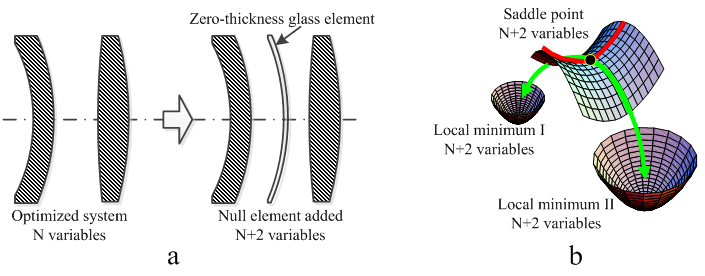
\includegraphics[scale=0.68]{FigSPCDemo.png}
    \caption{Illustration of SPC. (a) SPC with insertion of a zero-thickness glass meniscus. (b) A Morse index one saddle point in the 2D case.}
    \label{fig:SPCdemo}
\end{figure}

The pair of surfaces with equal curvatures can be either a zero-thickness lens added to the old minimum or a zero-thickness air space inside a lens of the old minimum. This added lens or air space will not affect the ray paths, and hence it will not affect the merit function value $MF_0$ of the original system. Therefore, such an element is called a null element. The two added variables are the surface curvatures $c_{N+1}$ and $c_{N+2}$ of the zero-thickness pair of surfaces. For any values of $c_{N+1} = c_{N+2}$ we can therefore write
\begin{equation} \label{eq:1}
    MF(\vec{v_0},c_{N+1},c_{N+2}) = MF_0 \textrm{, for } c_{N+1}=c_{N+2} 
\end{equation} 
where $MF$ is the merit function value of the system after adding the null element, and $\vec{v_0}$ is the vector of all variables of the minimum before insertion, which is kept constant.

In order to find the values of the null element curvatures for which the resulting system is an SP we must find the zeros of the partial derivative of the merit function with respect to the curvature of the null element. In a nutshell, the partial derivatives of the merit function with respect to the old optimization variables remain unchanged, hence they are all zero. Only the derivatives with respect to the new variables need to be considered
for finding the SP. In fact, because these two curvatures are not independent, annulling one of them is sufficient \cite{MVTurnhoutSPC15}. Therefore, if we denote $c_{N+1} = c_s$ to find curvature values for which the system is an SP we look for curvature values cs that satisfy the condition
\begin{equation} \label{eq:2}
    \frac{\partial}{\partial{c_s}} MF(\vec{v_0},c_s,c_{N+2}) \rvert_{c_{N+2}=c_s} = 0
\end{equation}
We solve Equation \ref{eq:2} with a numerical scan programmed in the macro language of CODEV. Since only two variables were added to the original minimum, the MI of this critical point cannot be larger than two. In all cases we have examined so far, the critical points we have found with SPC are only MI one SPs. Figure \ref{fig:SPCscan} shows an example of an SPC scan. There are four zero crossings in Figure \ref{fig:SPCscan} (b) indicating that four SPs are found. When the SPs are found, initial systems for subsequent local optimization can be obtained by choosing for each zero crossing in Figure \ref{fig:SPCscan} 2(b) two points, one to the left, one to the right of the crossing point. Local optimization, using, e.g., a damped-least square (DLS) algorithm, will then lead to two minimums, one on each side of the “saddle,” as shown in Fig \ref{fig:SPCdemo} (b). To obtain the broadest variety of new minimums with SPC, in general both zero-thickness lenses and zero-thickness airspaces may be necessary. For simple systems, there are examples of minimums that can be obtained with one of these two types of null elements but not with the other one. Finding the saddle points is in principle much less time consuming than DLS optimization, because it only involves the evaluation of the derivative of the MF for the 1D sequence of scan points according to Equation \ref{eq:2}, whereas local optimization involves many iterations where a Jacobian matrix is evaluated. The zero-thickness condition for the null element is not a severe limitation, as it may seem, because in the resulting minimums the distances between the surfaces (and the glass of the new lens) can be easily changed as desired. At this stage other parameters of the new lens (thickness, aspheric coefficients, etc.) can be made variable.

\begin{figure}[h!]
    \centering
    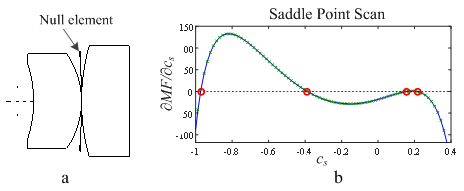
\includegraphics[scale=0.8]{SPCscan}
    \caption{Example of an SPC scan. (a) The insertion of a glass null element between two lenses of a known minimum. (b) The SPC scan finds four saddle points in this search. The red circles indicate the corresponding values of the null element curvatures.}
    \label{fig:SPCscan}
\end{figure}


The contents of the dissertation are included between the \texttt{\textbackslash begin\{document\}} and \texttt{\textbackslash end\{document\}} commands, and split into three parts by
\begin{enumerate}
\item\texttt{\textbackslash frontmatter}, which uses Roman numerals for the page numbers and is used for the title page and the table of contents;
\item\texttt{\textbackslash mainmatter}, which uses Arabic numerals for the page numbers and is the style for the chapters;
\item\texttt{\textbackslash appendix}, which uses letters for the chapter numbers, starting with `A'.
\end{enumerate}
The title page is defined in \texttt{title.tex} in the \texttt{title} folder and included verbatim with \texttt{\textbackslash include\{title/title\}},\footnote{Note that it is not necessary to specify the file extension.} (see below). Additionally, it is possible to include a preface, containing, for example, the acknowledgements. An example can be found in \texttt{preface.tex}. The table of contents is generated automatically with the \texttt{\textbackslash tableofcontents} command. Chapters are included after \texttt{\textbackslash mainmatter} and appendices after \texttt{\textbackslash appendix}. For example, \texttt{\textbackslash include\{chapter-1/chapter-1\}} includes \texttt{chapter-1.tex}, which contains this introduction.

\section{Title Page}

\dropcap{T}{he} title pages are defined in \texttt{title/title.tex}, which you will have to modify according to your needs. Note that these pages are subject to the requirements of the \emph{promotieregelement} and cannot be changed at will. Apart from the names and dates, most of the Dutch text is dictated literally.

Since the thesis title and name of the author appear several times throughout the document (on the title page, but also in, \emph{e.g.}, the preface and cv), special commands are provided so they only have to be specified once. The title (and optional subtitle) can be specified with

\begin{quote}
\texttt{\textbackslash title[Optional subtitle]\{Title\}}
\end{quote}
The name of the author is specified with
\begin{quote}
\texttt{\textbackslash author\{First name\}\{Last name\}}
\end{quote}
Note that the first and last name are separate arguments, since they may be printed in different font shapes. The \texttt{\textbackslash title} and \texttt{\textbackslash author} commands also ensure that the title and author appear in the metadata of the final PDF.

See \texttt{title/title.tex} for detailed documentation on the comment and layout of the title pages. Logos of institutes that have contributed financially to the dissertation may be included on reverse side of the title page. A few example logos can be found in the \texttt{title/logos} folder.

\section{Chapters}

\dropcap{E}{ach} chapter has its own file. For example, the \LaTeX{} source of this chapter can be found in \texttt{chapter-1.tex}. A chapter starts with the command

\begin{quote}
\texttt{\textbackslash chapter\{Chapter title\}}
\end{quote}
This starts a new page, prints the chapter number and title and adds a link in the table of contents. If the title is very long, it may be desirable to use a shorter version in the page headers and the table of contents. This can be achieved by specifying the short title in brackets:

\begin{quote}
\texttt{\textbackslash chapter[Short title]\{Very long title with many words which could not possibly fit on one line\}}
\end{quote}
Unnumbered chapters, such as the preface, can be created with \texttt{\textbackslash chapter*\{Chapter title\}}. Such a chapter will not show up in the table of contents or in the page header. To create a table of contents entry anyway, add
\begin{quote}
    \texttt{\textbackslash addcontentsline\{toc\}\{chapter\}\{Chapter title\}}
\end{quote}
after the \texttt{\textbackslash chapter} command. To print the chapter title in the page header, add
\begin{quote}
    \texttt{\textbackslash setheader\{Chapter title\}}
\end{quote}

If (parts of) the chapter have already been published elsewhere, it is customary to add a reference. This can be done with the special unnumbered footnote command \texttt{\textbackslash blfootnote}. For example,

\begin{quote}
\texttt{\textbackslash blfootnote\{Parts of this chapter have been published in Annalen der Physik \textbackslash textbf\{324\}, 289 (1906) \textbackslash cite \{Einstein1906\}.\}}
\end{quote}
generates the footnote at the beginning of this chapter. Because this footnote is unnumbered, the \texttt{hyperref} package may throw a warning, which safely be ignored.

If multiple people have contributed significantly to this chapter, they can be lister with the \texttt{\textbackslash authors} command. This can be followed by a quotation using \texttt{\textbackslash epigraph} as shown above. Finally, it is customary for a dissertation to include an abstract for every chapter (except perhaps the introduction). This can be accomplished with the \texttt{abstract} environment. The abstract should be followed by \texttt{\textbackslash newpage} to start the chapter text on a new page.

In a dissertation, each chapter has its own list of references. These can be generated with the special command \texttt{\textbackslash references\{dissertation\}} from \texttt{dissertation.bib} at the end of the chapter. Note that this means that you need to run a command like \texttt{bibtex chapter-1/chapter-1} for each chapter. The bibliography style is specified in \texttt{dissertation.bst}, which is a modified version of \texttt{apsrev4-1.bst} (from REVTeX) designed to also display the titles of referenced articles. The template will automatically generate clickable hyperlinks if a URL or DOI (digital object identifier) is present for the reference. Although it is possible to manage the bibliography by hand, we recommend using EndNote (available from Blackboard) or JabRef (available from \url{http://jabref.sourceforge.net/}).

Chapters are subdivided into sections, subsections, subsubsections, and, optionally, paragraphs and subparagraphs. All can have a title, but only sections and subsections are numbered. As with chapters, the numbering can be turned off by using \texttt{\textbackslash section*\{\ldots\}} instead of \texttt{\textbackslash section\{\ldots\}}, and similarly for the subsection.
\section{\textbackslash section\{\ldots\}}
\subsection{\textbackslash subsection\{\ldots\}}
\subsubsection{\textbackslash subsubsection\{\ldots\}}
\paragraph{\textbackslash paragraph\{\ldots\}}
Lorem ipsum dolor sit amet, consectetur adipisicing elit, sed do eiusmod tempor incididunt ut labore et dolore magna aliqua. Ut enim ad minim veniam, quis nostrud exercitation ullamco laboris nisi ut aliquip ex ea commodo consequat. Duis aute irure dolor in reprehenderit in voluptate velit esse cillum dolore eu fugiat nulla pariatur. Excepteur sint occaecat cupidatat non proident, sunt in culpa qui officia deserunt mollit anim id est laborum.

\section{Fonts and Colors}

\dropcap{T}{he} fonts used by this template depend on which version of \LaTeX{} you use. Regular \LaTeX, \emph{i.e.}, if you compile your document with with \texttt{latex}, \texttt{pslatex} or \texttt{pdflatex}, will use Utopia for text, Fourier for math and Latin Modern for sans-serif and monospaced text. However, if you want to adhere to the TU Delft house style, you will need to use \XeLaTeX, as it supports TrueType and OpenType fonts. Compiling with \texttt{xelatex} will use Bookman Old Style for titles, Tahoma for text, Courier New for monospace and Cambria for math. If you want to use \XeLaTeX, but do not want to use the TU Delft house style fonts, you can add the \texttt{nativefonts} option to the document class.

This template supports the use of drop caps, a large colored initial at the beginning of a chapter or section, via the \texttt{\textbackslash dropcap} command:

\begin{quote}
\texttt{\textbackslash dropcap\{L\}\{orem\} ipsum\ldots}
\end{quote}
The first argument is the capital that will be printed on two lines (in the title color), and the second argument is the rest of the word. Depending on the font, the latter may be printed in small caps.

The corporate colors of the TU Delft are cyan, black and white, available, respectively, via \texttt{\textbackslash color\{{\color{tudelft-cyan}tudelft-cyan}\}}, \texttt{\textbackslash color\{{\color{tudelft-black}tudelft-black}\}} (which differs slightly from the default \texttt{black}) and \texttt{\textbackslash color\{tudelft-white\}}. Apart from these three, the house style defines the basic colors
\begin{itemize}
%% Reduce the separation between the items, since this is just a list of words.
\itemsep 0pt
\parskip 0pt
\item\texttt{\color{tudelft-sea-green}tudelft-sea-green},
\item\texttt{\color{tudelft-green}tudelft-green},
\item\texttt{\color{tudelft-dark-blue}tudelft-dark-blue},
\item\texttt{\color{tudelft-purple}tudelft-purple},
\item\texttt{\color{tudelft-turquoise}tudelft-turquoise} and
\item\texttt{\color{tudelft-sky-blue}tudelft-sky-blue},
\end{itemize}
as well as the accent colors
\begin{itemize}
\itemsep 0pt
\parskip 0pt
\item\texttt{\color{tudelft-lavendel}tudelft-lavendel},
\item\texttt{\color{tudelft-orange}tudelft-orange},
\item\texttt{\color{tudelft-warm-purple}tudelft-warm-purple},
\item\texttt{\color{tudelft-fuchsia}tudelft-fuchsia},
\item\texttt{\color{tudelft-bright-green}tudelft-bright-green} and
\item\texttt{\color{tudelft-yellow}tudelft-yellow}.
\end{itemize}

\references{dissertation}


\setlength{\parskip}{.2em}
\graphicspath{ {./chapter-3/figures/} }
\captionsetup[figure]{labelfont=bf}
\captionsetup{margin=1.5em}
\captionsetup[table]{labelfont=bf}


\chapter{Lens Design Landscape Exploration with Simple Systems}
\label{chapter_SPC_simple_system_landscape}

%% The following annotation is customary for chapter which have already been
%% published as a paper.
\blfootnote{Parts of this chapter have been published in Applied Optics \textbf{55}, 10449 (2016) \cite{HouSimple16}.}

%% It is only necessary to list the authors if multiple people contributed
%% significantly to the chapter.
%\authors{Albert {\titleshape Einstein}}

% %% The '0pt' option ensures that no extra vertical space follows this epigraph,
% %% since there is another epigraph after it.
% \epigraph[0pt]{
%   A journey of a thousand miles begins with a single step
% }{Laozi}

% \epigraph{
%     Sample quotes
% }{author}

% \begin{abstract}
% Previous researches have shown that different solutions of the optical system can be found using saddle point based method for some simplified cases\cite{PascalTriplet2009}. It is important, however, to study whether the saddle point based method still perform well in practical lens design problems. To study this, we chose to start with a relative simple example.
% \end{abstract}

% %% Start the actual chapter on a new page.
% \newpage

\noindent 
In a lens design landscape, from a saddle point system with Morse index $1$, optimization will lead to two solutions of local minima.  When performing a SPC \footnote{The definition of "performing an SPC scan" is given in Chapter \ref{spc-general}.}, it can find several saddle point configurations, which subsequently lead to multiple local minima. 

Therefore, it is an intriguing question whether or not the local minima in the design landscape are all connected by the saddle points of Morse index $1$. If this is the case, then by constructing sufficiently many saddle points, in principle all local minima of the design landscape can be obtained. 

This chapter is mainly based on a research paper\cite{HouSimple16} published in 2016. It is shown that in the design landscape of a wide-angle pinhole lens and in closely related optimization landscapes, all good local minima found by other methods can be obtained easily with a succession of one-dimensional searches (SPC scans) starting from simpler systems. By replacing high-dimensional searches with a succession of one-dimensional searches, the design efficiency can be increased significantly. By combining this method with conventional design methods, the wide-angle pinhole lens can be designed starting from a single lens.

% Reason for choosing the wide-angle pinhole lens. 1) Application wise, it is application wise popular. 2) It is sufficiently different from the previous studied ideal examples.
In a 2004 research paper \cite{BociortThinLens2004}, Bociort et al. show that when some general mathematical requirements are satisfied, %{a thin lens model is used, and only the spherical aberration is considered, }
the minima and saddle points in the lens design landscape form a network. The saddle points in this network can be theoretically predicted, hence from the saddle points, minima are obtained. Research conducted by Van Grol et al.\cite{PascalTriplet2009} claims that there is a fundamental network for a lens design problem with a certain number of lenses. In their paper, examples of the fundamental network of doublet and triplet systems are given. The authors predict that in practical design cases, the types of system shapes \footnote{In a lens system, each lens element has its lens form: biconcave, biconvex, meniscus, etc. The type of the system shape of a lens system is determined by the combination of the individual lens forms. For example, a biconcave-biconvex doublet is one type of system shape, and a biconcave-meniscus is a different type of system shape. } of the solutions will not exceed the types of system shapes from the fundamental network. In a later paper from 2010\cite{BociortTripletExplained2010}\cite{BociortToyModel2010}, Bociort shows that a toy model based on third-order spherical aberration can be used to mathematically explain the fundamental network of the triplet. 

For the assumption that the dominant aberration is spherical aberration, and that the lenses are not too thick, it is possible to predict the existing solutions within the network. However, in practical cases, aberrations other than spherical aberration will also determine the topology of the merit function landscape. In this case, it is mathematically too complex to build an analytical model to predict the behaviour of the merit function landscape.

Despite the complexity to use an analytic model to predict the merit function landscape, earlier research shows \cite{BociortSPCSexplained}\cite{MVTurnhoutSPC15} that in the lens design space, a special structure is present that makes the lens design problem different from a general global optimization problem: certain saddle points existing in the landscape are reducible to minima of simpler systems with one lens element less. Using this structure, the SPC \cite{MVTurnhoutSPC15} method is developed to obtain new design solutions. In the conventional approach, trial and error is needed to look for different solutions (if there is more than one) by adding one extra lens element to the existing system. With the SPC, there is a systematic procedure to search for available solutions by adding new elements to the system. When starting from a minimum with $N$ variables, with SPC it is possible to systematically find minima in an $(N+2)$-dimensional variable space by using one-dimensional searches, rather than $(N+2)$-dimensional searches. Important questions are, however, how many minima existing in the landscape can be obtained in $(N+2)$-dimensional search spaces, by replacing high-dimensional searches with one-dimensional searches? What percentage of them can be found? Is it possible to at least obtain the good solutions? In this chapter, the performance of SPC is evaluated for more general problems, especially those of practical interests. 


%%%%%%%%%%%%%%%%%%%%%%%%%%%%%%%%% Section 1 %%%%%%%%%%%%%%%%%%%%%%%%%%%%%%%%%%%%%%%
\section{Wide-angle Pinhole Lens}

A wide angle pinhole lens, designed by Irina Livshits from ITMO, has been chosen to study the design landscape using SPC. For surveillance applications, this kind of lens, has in recent years, become very popular. Instead of a lensless optical element, the pinhole lens here refers to a lens having an aperture stop with a small diameter placed in front of the system. All lenses are in contact, one lens is cemented, and three different glass materials are used [see Figure \ref{fig:widepinLens}(a)]. The design specifications are given in Table \ref{table: sysspec} and the surface specifications are provided in Appendix \ref{apdx: wide-angle-specs_4_elements}. In Figure \ref{fig:widepinLens}(b) a 2D image simulation made with CODE V shows that, despite its simplicity, the system has an imaging quality that is adequate for its intended purpose. The system can also be adapted for spectral imaging applications \cite{Strauch2015}. For optimization we use the default CODE V merit function that is based on transverse ray aberrations. The value of the merit function (called in CODE V error function) for this system is 5.68 \textmu m$^2$. It is a composite value, scaled so that it is the mean square of the weighted image radius. The value has considered a setting with three wavelengths as shown in Table \ref{table: sysspec}. In the following text in this chapter, values of the merit function are presented without adding the unit. 

\begin{figure}[h!]
    \centering
    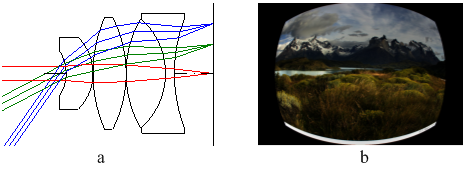
\includegraphics[scale=0.95]{chapter-3/figures/WidePinLens.png}
    \caption{Wide-angle pinhole lens. (a) Lens drawing. (b) 2D image simulation of its imaging quality.}
    \label{fig:widepinLens}
\end{figure}

\setlength{\arrayrulewidth}{.5mm}
\setlength{\tabcolsep}{18pt}
\renewcommand{\arraystretch}{1.2}
\begin{table}[h!]
    \centering
    \captionsetup{justification=centering}
    \caption{System specification}
    \label{table: sysspec}
    \vspace{-1em}
    \begin{tabular}{ p{20em} c }
    \hline 
    Entrance Pupil Diameter (EPD, mm) & 0.8\\
    (Full) Field Of View (FOV, °) & 110\\
    Effective Focal Length (EFL, mm) & 3.5\\
    Wavelength (nm) & 644, 546, 480\\
    \hline
    \end{tabular}
\end{table}



%%%%%%%% SECONTION Switching %%%%%%%%%%%%%%%%%%%%%%%
\section{Switching Between Local Minima}

To find other possible solutions for the same specifications, two different global optimization methods are used, Global Synthesis from CODE V \cite{KuperGO1992}\cite{RogersGO2006} and a saddle point detection method (the program NETMIN\footnote{NETMIN is a tool developed in TU Delft to search for new local minima based on saddle point detection method. Detailed description can be found in Chapter \ref{method: spd}.}). In this example, for simplicity only the surface curvatures are used as variables. Minor edge thickness violations, which can be easily corrected in a later stage, are acceptable in this analysis. 

It is of interest to find the so-called stable solutions, i.e., the solutions that do not easily appear or disappear when specifications are slightly changed. Three stable solutions are found, denoted in Figure \ref{fig:wideangleSwitch} by M1, M2, and M3. They exist for a wider range of specifications, e.g., not only for the field of view (FOV) of 110° as shown in Table \ref{table: sysspec}, but also for a FOV of 90°, and not only for an effective focal length (EFL) of 3.5 mm (for which the corresponding merit function values are 5.68, 11.51, and 11.09, respectively) but also for an EFL of 3.0 mm (with merit function values of 6.80, 23.20, and 16.70). These solutions have no large edge thickness violation and relatively low merit function values. From the lens drawings of these solutions, we observe that the second element differs significantly between them. A few solutions with low stability and large merit function values can also be found. They exist for instance either at EFL 3.5 mm or at EFL 3.0 mm, but not at both. Since these solutions with low stability appear or disappear easily when the EFL is changed, it is reasonable to assume that their basins of attraction (i.e., the set of starting points in the variable space that after optimization converge to the given solution) are small and therefore the risk that the optimization gets trapped in these basins is rather low. The solutions with low stability will therefore be ignored in what follows. While no global optimization method can guarantee that all minima are found, the landscapes examined in this research are simple enough so that there is a high probability that all minima having a basin of attraction large enough to be relevant, are found with the methods being used. 

\begin{figure}[h!]
    \centering
    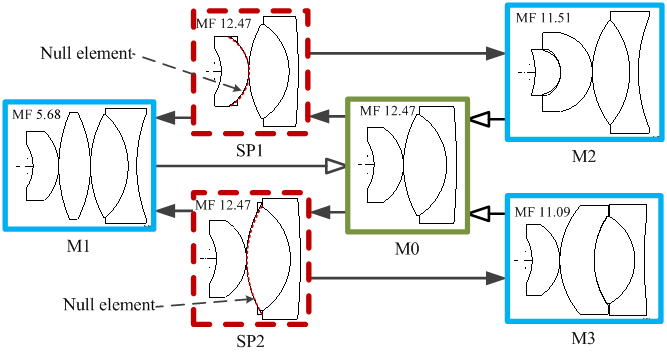
\includegraphics[scale=0.6]{chapter-3/figures/WideAngleSwitch.png}
    \caption{Switching between minima (blue boxes) using SPC. Extraction of the second element from M1, M2, or M3 results in the system M0 (hollow arrows). Starting from M0, two routes, each having an SP, lead to three different minima (solid arrows). The two saddle points shown in dashed red boxes can be found both by the general and by the special version of SPC. In SP1, the null-element has the same curvature as the second surface of M0; in SP2, it has the same curvature as the third surface of M0 (because of two zero thicknesses, we see there three overlapping surfaces, marked by red dashed line).}
    \label{fig:wideangleSwitch}
\end{figure}

Optimization can be trapped in the sub-optimal minima M2 and M3, which are significantly worse than M1. However, the global minimum M1 can be rapidly obtained with SPC from both of them. In M2 or M3, the second element is extracted first and then the SPC method is applied (suitable candidate lenses for extraction are in general weaker-power lenses that seem to have little function). After extraction and optimization, both solutions become the M0 system shown in the green box in Figure \ref{fig:wideangleSwitch} Then two saddle point systems, SP1 and SP2 in Figure \ref{fig:wideangleSwitch} (in the red dashed boxes), were constructed from M0 by adding a null element in between the first and the second lens (i.e., at the position of extraction). From each saddle point system, two local minima can be found after optimization. In this case, both saddle point systems lead on one side to the same minimum, the global minimum M1. On the other sides, the two saddle points lead to M2 and M3. In fact, from any of these three minima, the other two can be found by a switching operation. In this example, different ways of using the SPC method described in Chapter 2 are demonstrated: firstly, the SPC method can systematically find new solutions with more lenses (M1, M2, and M3) from a simpler system (M0); secondly, extracting and then adding lenses with the SPC can lead to different minima in a systematic way. This possibility of switching between different local minima is a typical property of the SPC.
%%%%%%%%%%%%%%%%%%%%%%%%%%%%%%%%%%%%%%%%%%%%% Section %%%%%%%%%%%%%%%%%%%%%%%%%%%%%%%%%%%%%%%%%%%%%%%%
\section{Designing a Pinhole System Starting from a Single Lens} \label{chrom90d}

In the previous section, by using SPC, we show how different designs can be found systematically by increasing the number of lenses. By using this approach in combination with traditional methods, it is possible to design an optical system starting with just one lens. This part shows how a pinhole lens similar to the one in Figure \ref{fig:widepinLens}(a) can be obtained from a single lens. The specifications are listed in Table \ref{table: sysspec}. The same merit function as before, is used.

A global optimization is performed starting from a plane parallel plate. Only one singlet solution is obtained, with a merit function value of 576.30, as shown on the left in Figure \ref{fig:WideAngleDesign}(a). This singlet serves as a basic element, providing optical power to the system \cite{LivshitsQA2013}. On this singlet, SPC is performed by adding a zero-thickness glass element at the back surface. Two doublet minima are found, with merit function values 164.81 and 1783.94 (the latter one disappears if we replace EFL 3.5 mm by, e.g., EFL 3.0 mm). The better one (the first one) is chosen for the next design step. 

\begin{figure}[h!]
    \centering
    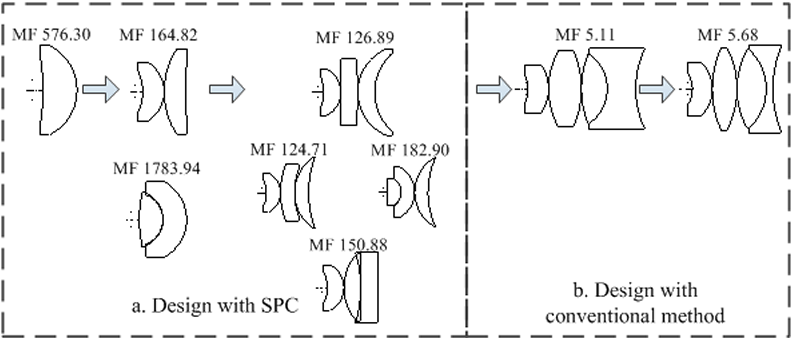
\includegraphics[width=1.0\textwidth]{chapter-3/figures/WideAngleDesign.png}
    \caption{Designing a wide-angle pinhole lens from one lens by combining SPC with conventional methods.}
    \label{fig:WideAngleDesign}
\end{figure}

With the same strategy, SPC is performed on four different surfaces of the doublet with a merit function value of 164.82 and four triplet minima are found (with merit function values 124.71, 126.89, 150.88, and 182.90, respectively). Only one type of glass is used for the steps mentioned above. In the next step, we continue with the best two minima using conventional design techniques: glasses are changed and the third lens is replaced with a cemented doublet to correct chromatic aberrations. The glasses are selected to be the same as the original system designed by Irina Livshits. When the glass are modified, the best minimum (a merit function value of 124.71) of the triplets encounters ray failure. However, the system with a merit function value of 126.89 still remains stable after changing the glass. Optimization with all curvatures and thicknesses as variables leads to a system with a merit function value of 5.11 [Figure \ref{fig:WideAngleDesign}(b)]. By readjusting the thickness of the lenses for a more compact size, a system with the merit function value of 5.68 was obtained [see Figure \ref{fig:WideAngleDesign}(b)], which is identical to the original design in Figure \ref{fig:widepinLens}(a).

SPC is useful for dealing with minima created by monochromatic aberrations. It cannot deal directly with minima created by chromatic aberrations. However, since typically chromatic aberrations are less non-linear than monochromatic ones (e.g., unlike the Seidel aberrations, for axial chromatic aberration the thin-lens expressions are linear), the chromatic aberrations tend to create fewer new minima than the monochromatic
ones. As shown in this example, in the design process SPC can be easily combined with traditional approaches to handle chromatic correction.

In addition, four triplet minima are found with the SPC method in the search using only one glass, as shown in Figure \ref{fig:WideAngleDesign}(a). Both Global Synthesis \footnote{It is a proprietary global optimization algorithm of CODE V. The algorithm starts from the given system and explore solutions space for new configurations in a systematic manner.} and saddle point detection
(NETMIN) finds only three minima (missing the one with the merit function value of 182.90). Therefore in this example, the SPC method has the advantage of being able to find more minima than the two methods used for comparison. 

%%%%%%%%%%%%%%%%%%%%%%%%%%%%%%%%%%%%%%%%%%%%% Section %%%%%%%%%%%%%%%%%%%%%%%%%%%%%%%%%%%%%%%%%%%%%%%%
\section{Decomposing a High-dimensional Search for New Minima in a Succesion of One-dimensional Searches}  \label{chrom60d}

It is mentioned in the previous section that the SPC found more system candidates compared to the Global Synthesis of CODE V and the saddle point detection algorithm. However in the examples, the number of minima found in the landscape is small. In this section it is investigated whether the performance of SPC is still good when more minima are present in the landscape.

In order to generate more minima, the FOV of the triplet system is reduced to 60° while the other specifications remained as that given in Table \ref{table: sysspec}. The reason why a reduced
field leads to more minima will be discussed in the next section.
As in Figure \ref{fig:WideAngleDesign}(a) only one type of glass is used, the variables are only the curvatures. The same default CODE V merit function is used, and, for the purpose of this study, the control of edge thickness is disabled. All lenses are in contact (i.e., all air spaces between lenses have zero thickness). The thicknesses of all lenses in a minimum system are set equal in order to avoid the multiple appearance of essentially the same minima (with similar curvatures, but different lens thicknesses) that would unnecessarily complicate the study \cite{HouProc2015}.

For a better understanding of the results, in addition to the comparison of minima, it is also useful to compare the saddle points obtained using SPC with those obtained using the saddle point detection algorithm (realized by the program NETMIN). For SPC there are the options of inserting in the existing minimum either a glass null-element (i.e., inserting a lens) or an air null-element (i.e., splitting a lens). If the zero-thickness glass element was used, the saddle points resulting from the SPC scan would still have a zero-thickness lens, whereas the saddle points detected with NETMIN would have finite thicknesses for all lenses. This is because that the NETMIN starts from existing minima with non-zero thickness element and searches for the saddle points. The saddle points obtained from the two methods can not be directly compared due to the thickness differences of the lens element. In our study, all lens elements are set to be in contact. In this case, the saddle points detected with NETMIN will have zero air spaces. It is therefore better for comparison to study the performance of the SPC when air null elements are used. Splitting lenses with SPC leads to saddle points with a zero distance between lenses, which are directly comparable with the saddle points from NETMIN. For performing SPC with a zero-thickness air element, the thickness of the lens, which will be split, is first doubled. Then the system is re-optimized to a minimum, and a zero-thickness air element is inserted in the middle of the lens. As mentioned in section \ref{section: SPC recommendation}, the example of Cooke triplet shows that the minima are different between applying zero-thickness glass and zero-thickness air space constructions. Therefore, both approaches are recommended to be used. However, in this example, it turns out that SPC with zero-thickness glass does not give more local minima than using zero-thickness airspace. For simplicity and better comparison, the SPC result using zero-thickness air space is shown. 
\begin{figure}[h!]
    \centering
    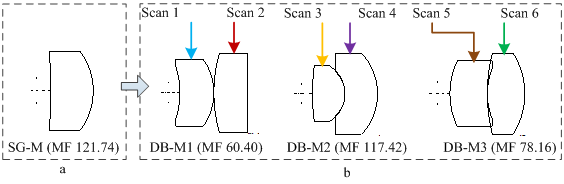
\includegraphics[width=0.8\textwidth]{chapter-3/figures/Single2Double.png}
    \caption{SPC by inserting a zero-thickness air element. (a) Singlet solution (SG-M). (b) The three doublet minima (DB-M) that result from the singlet are the starting minima for the scans shown in Figure \ref{fig:tripletnetwork}.}
    \label{fig:single2double}
\end{figure}

As previously, we start with a single optimized lens [SG-M shown in Figure \ref{fig:single2double}(a)] and three doublets are obtained with the SPC [shown in Figure \ref{fig:single2double}(b)]. The three doublets DB-M1, DB-M2, and DB-M3 have a total of six lenses.  Each of the six lenses is used to generate an SPC scan which leads to triplet minima. The colored arrows in Figure \ref{fig:single2double}(b) indicate the lenses that are split (after the thickness doubling that is not shown here) in the corresponding scan.

Figure \ref{fig:tripletnetwork} shows the minima and saddle point systems found in the triplet design space with NETMIN and Global Synthesis (Global Synthesis has found nine out of 10 minima, missing the minimum M6). Five curvatures are used as variables, and the curvature of the last surface is controlled by a \textit{Solve} in CODE V to keep the effective focal length constant.

A significant result of this search is that all 10 triplet minima shown in Figure \ref{fig:tripletnetwork} are also obtained with SPC starting from the three doublets in Figure \ref{fig:single2double}. Eleven saddle point systems are obtained from the six one-dimensional SPC scans. Different scans find different numbers of saddle points. For instance, in Scan 2 there are four saddle points (SP1, SP2, SP7, and SP8 in Figure \ref{fig:tripletnetwork}), whereas in other scans, only one or two saddle points are found. The 10 minima are resulted from the 11 saddle point systems by optimising on both sides of the saddle. Saddle point systems and minima obtained from the same scan are connected in Figure \ref{fig:tripletnetwork} with the same colored lines. In the figure, when we gradually increase the FOV, M1 corresponds to the system leading to the final design in the 110° case [merit function value 126.89 in Figure \ref{fig:WideAngleDesign}(a)]. However, in this case, its merit function value of 61.14 is not the smallest one in Figure \ref{fig:tripletnetwork}.

NETMIN finds the extra saddle point system SP12, which cannot be found by SPC. This saddle point system connects with a dashed link the minima M3 and M9 in Figure \ref{fig:tripletnetwork}. However, there is sufficient redundancy in the SPC approach, and both M3 and M9 also result from other saddle point systems which are found by SPC. Therefore the lack of ability of SPC to find SP12 is not critical.

Since there are five variables, with general global optimization tools this search has to be performed in a five-dimensional space. In this example, however, all minima found with other methods are also found with SPC, where the five-dimensional search is replaced by six one-dimensional searches. Replacing a high-dimensional search for new minima by a succession of one-dimensional searches reduces the complexity of the search significantly.

The example discussed above shows the utility of the feature of the optical merit function landscape that enables the decomposition of the search for many of the minima in simpler steps. The feature means that minima and saddle points are all connected, and the saddle points can be constructed by SPC. This example has the advantage that in this case, the feature mentioned above can be observed in a pure form, without interference from other features (e.g. the minima are not connected by saddle points that can be constructed) of the landscape. However, in general, other features which deserve further study to gain a better understanding, may also play a role. Therefore, it cannot be expected that we can always find all minima using SPC. Nevertheless, even when other features are present, examples studied so far show that SPC can lead to satisfactory results.

For instance, when the search described in Figure \ref{fig:tripletnetwork} is repeated with modified wavelength specifications, SPC finds 11 minima and Global Synthesis finds 10 (see Figure \ref{fig:TripletMonoNetwork}). Among these minima, eight, including the best five, are found by both methods. For the four minima that are missed by SPC, two of them are unphysical (minima 12 and 14, they have either negative or zero back focal length that cannot be corrected, but should be prevented with an additional constraint). These unphysical solutions also have a merit function more than 4 times and more than 50 times that of the best solution. The other two minima missed by SPC (minima 13 and 15) have merit function values 40 times and 8 times that of the best solution. NETMIN finds all four solutions missed by SPC, and Global Synthesis finds two of them.

% \begin{figure}[h!]
%   \begin{adjustbox}{addcode={%
%     \begin{minipage}{\width}}{%
%     \captionsetup{margin=0em}
%     \caption{Network of minima (solid boxes) and SP systems (dashed boxes) in the 60° landscape, where the other specifications are the same as in Table \ref{table: sysspec}. Eleven SP systems result from six SPC scans (each color represents one scan). Optimization starting at these SP systems leads to all 10 minima that were obtained with NETMIN and Global Synthesis. If in any of these 11 SPs we remove the null-element of the corresponding scan (this does not affect the ray paths or the MF), we obtain the starting doublet of the scan. The null elements are marked by crosses with the corresponding color. This figure shows why the lens design landscape is different from general global optimization landscapes: because of the close relationship that exists between local minima of a design problem (here the 10 triplet minima) and local minima with one lens less (here the starting doublets).}\label{fig:tripletnetwork}
%     \end{minipage}},rotate=90,center}
%     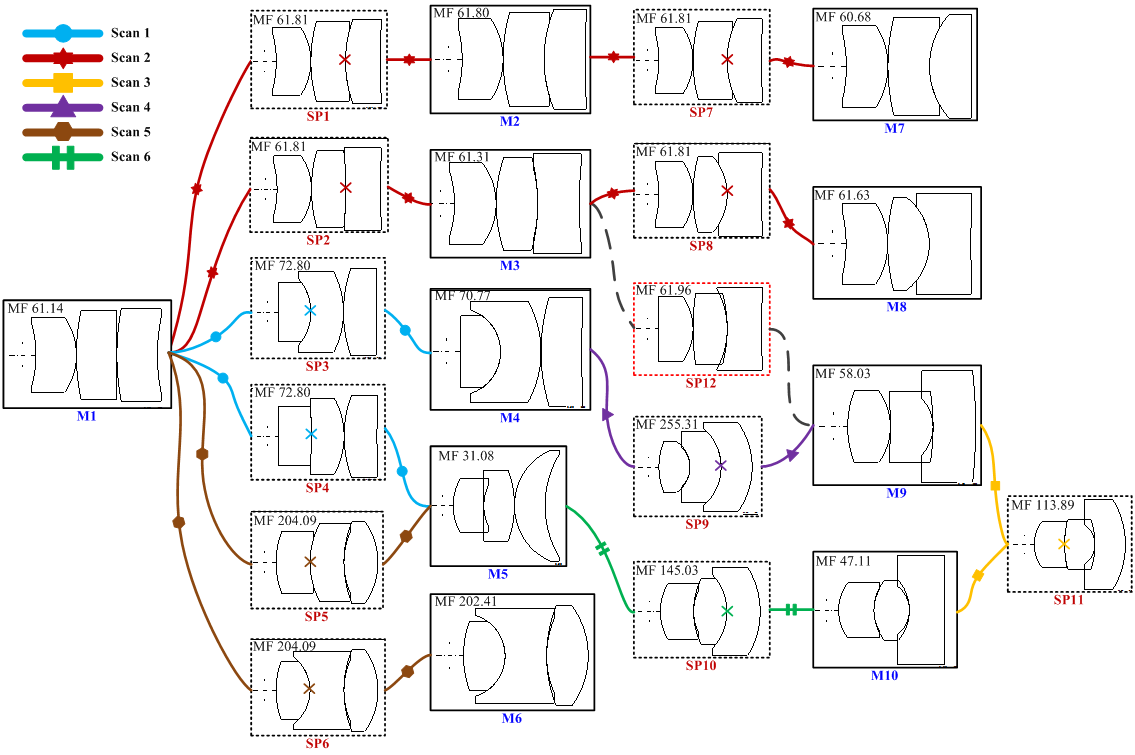
\includegraphics[scale=0.5]{chapter-3/figures/TripletNetwork.png}
%   \end{adjustbox}
% \end{figure}

\begin{figure}[h!]
    \centering
    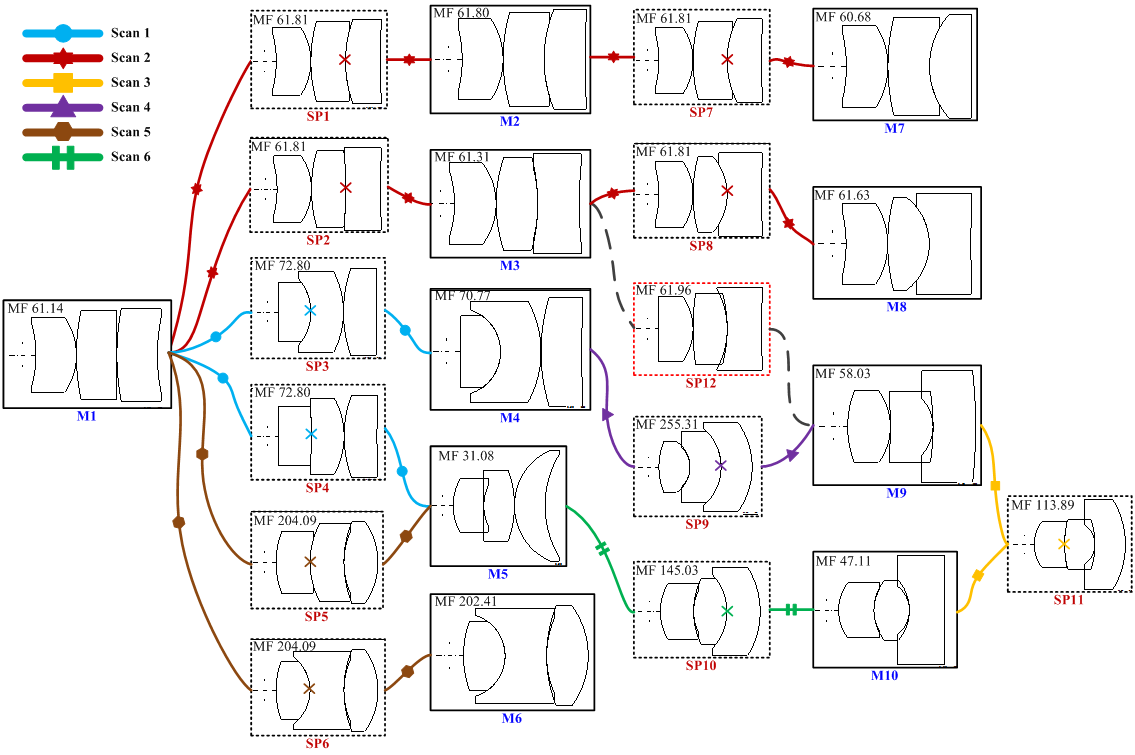
\includegraphics[scale=0.41]{chapter-3/figures/TripletNetwork.png}
    \caption{Network of minima (solid boxes, named as M\#) and saddle point systems (dashed boxes, named as SP\#) in the 60° landscape, where the other specifications are the same as in Table \ref{table: sysspec}. Eleven saddle point systems result from six SPC scans (each color represents one scan). Optimization starting at these saddle point systems leads to all 10 minima that are obtained with NETMIN and Global Synthesis. If in any of these 11 saddle points we remove the null-element of the corresponding scan (this does not affect the ray paths or the merit function), we obtain the starting doublet of the scan. The null elements are marked by crosses with the corresponding color. This figure shows why the lens design landscape is different from general global optimization landscapes: because of the close relationship that exists between local minima of a design problem (here the 10 triplet minima) and local minima with one lens less (here the starting doublets).}\label{fig:tripletnetwork}
\end{figure}

Despite the fact that SPC cannot find four (poor-quality) minima directly, it turns out that by using the switching strategy described earlier, it is easy to escape from any of them if optimization is trapped. Eliminating a lens from any of these poor-quality minima leads to one of the three doublets. From these doublets, better minima can be obtained with SPC.
\begin{figure}[h!]
    \centering
    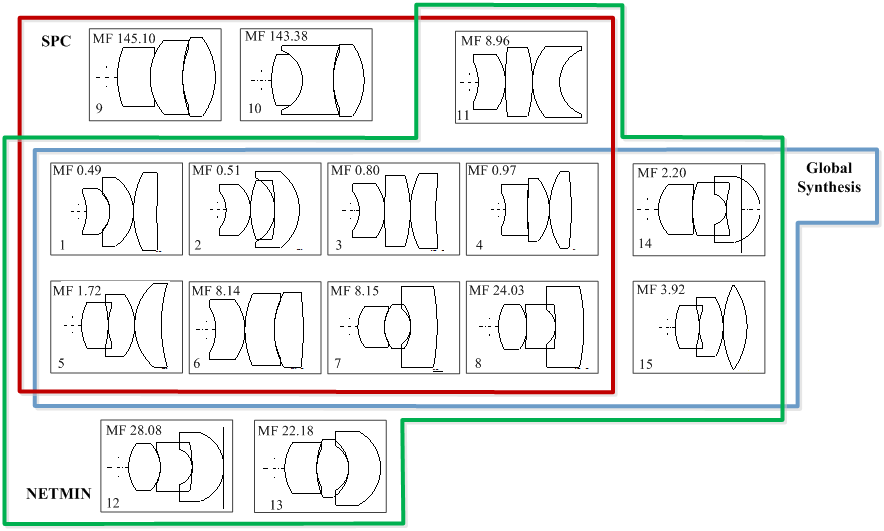
\includegraphics[width=1.0\textwidth]{chapter-3/figures/TripletMoNoNetwork.png}
    \caption{Minima found with SPC (red box), Global Synthesis (blue box), and NETMIN (green box) in a monochromatic run. Minima 12 with Merit Function (MF) value 28.08 and Minima 14 with MF value 2.20, whose image planes are inside or coincide with the last lens, are unphysical. The five minima with the lowest MF value (numbered from 1 to 5) are found by all three methods. Edge thickness violations is disabled in this search.}
    \label{fig:TripletMonoNetwork}
\end{figure}

However, in order to understanding the potential and the limitations of SPC, it is useful to examine why SPC is not able to reach these four minima. SPC is based on the assumption that small changes in lens thicknesses do not affect good designs significantly, i.e., that good minima continue to exist as minima when a reasonably small non-zero thickness is replaced by zero. This assumption is similar to the one at the basis of the well-known thin-lens aberration theory. In earlier days of lens design, primary aberration formulas using zero thickness were used to qualitatively predict the existence of good designs.

It turns out that the minima that are not found by SPC only exist for certain non-zero thickness values and do not have a zero-thickness equivalent. However, the existence of these minima does not contradict our assumption that using SPC can obtain satisfactory solutions, because these are not among the best solutions. In the numerical experiment, final solutions have the same thickness for each lens element (1.5 mm). Since in the SPC procedure the practical design is always obtained after increasing the zero-thickness of a null element, it is not possible to reach minima that disappear when the lens corresponding to the null element has zero thickness. In NETMIN and Global Synthesis searches, the lens thicknesses are kept constant. This typical behavior is illustrated in Figure \ref{fig:thicknesschange}(a) and (b). In the system in Figures \ref{fig:thicknesschange}(a) found by SPC, the thickness of the first lens is 1.5 mm. By starting with a zero-thickness null-element as the first lens as in Figure \ref{fig:thicknesschange}(b), increasing the thickness leads to the system in Figure \ref{fig:thicknesschange}(a). By decreasing the thickness of the first lens of the system in Figure \ref{fig:thicknesschange}(a), the system in Figure \ref{fig:thicknesschange}(b) is obtained. In contrast, in the system in Figure \ref{fig:thicknesschange}(c) found by NETMIN but not by SPC, when the thickness of the first lens is decreased ray failure occurs and a system with zero-thickness element cannot be obtained. However, systems like the one in Figure \ref{fig:thicknesschange}(c) have low stability. A small perturbation on the system in Figure \ref{fig:thicknesschange}(c) will lead to the system in Figure \ref{fig:thicknesschange}(a).

\begin{figure}[h!]
    \centering
    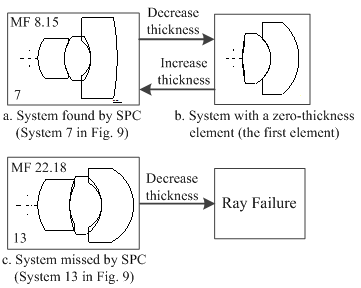
\includegraphics[scale=0.7]{chapter-3/figures/thicknesschange.png}
    \caption{Increasing the thickness of the first element of system (b) results in system (a), and vice versa. System (b), which is obtained by the SPC, is a minimum with a zero-thickness element. System (c), which is missed by the SPC, does not have a corresponding zero-thickness pair. A small perturbation on system (c) will lead to system (a).}
    \label{fig:thicknesschange}
\end{figure}


%%%%%%%%%%%%%%%%%%%%%%%%%%% Section %%%%%%%%%%%%%%%%%%%%%%%%%%%%%%%%%%%%%%%%%%%
\section{Effect of Changing the Field of View on the Landscape}
In Section \ref{chrom90d} and \ref{chrom60d} it is found that when the field of view is reduced, more minima can be found in the design space. This happens for two reasons. First, when design specifications (e.g., FOV or EPD) are modified, the distances in the design space between minima and saddle points change
and therefore the merit function landscape also changes. As can be observed in numerical experiments, when a minimum and a saddle point with Morse Index $1$ collide, they both disappear. Alternatively, such a pair can appear when specifications are changed. Similarly, two minima with a saddle point between them can be replaced by one minimum, and two saddle points with a minimum between them can be replaced by an SP. This can be explained mathematically by the conservation of the topological degree of the merit function landscape \cite{vanTurnhoutThesis2009} \cite{KoornwinderTopologicaldegree}. The topological degree of a critcal point is the sign of the determinant of the Hessian matrix in that point. The degree of a critical point is thus $(-1)^{Morse Index}$. A minimum has a topological degree of $+1$ and a saddle point with Morse Index $1$ has a topological degree of $-1$. The sum of the topological degrees remain constant under perturbation such as changing the FOV. Second, when the FOV is increased ray failure appears more easily, and the region of ray failure expands in the design space. Because certain minima and saddle points which exist for lower FOV cross the border of the ray failure region and disappear, fewer of them are found at large FOV.

 When varying the FOV of the systems shown in Figure \ref{fig:tripletnetwork}, the number of solutions changes with the FOV as shown in Figure \ref{fig:FOVvarying}. Three different FOVs are chosen: 110°, 90° and 60°. Six solutions were obtained for 110°, five for 90° and ten for 60°. From Figure \ref{fig:FOVvarying}, it is seen that some system shapes exist in all the three FOV configurations. However, other system shapes only exist in the specific FOV range.
For FOV 60°, five new systems, which did not exist for a larger field (second row for the 60° systems in Figure \ref{fig:FOVvarying}). The dashed boxes in Figure \ref{fig:FOVvarying} mark the missing systems which exist in other FOV specifications. As mentioned in the previous paragraph, the appearance and disappearance of the systems can be explained by the change of the merit function landscape. 

\begin{figure}[h!]
    \centering
    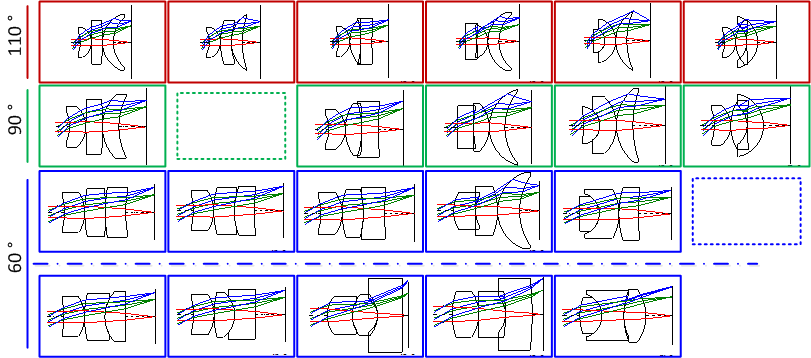
\includegraphics[width=1.0\textwidth]{chapter-3/figures/FOVvarying.png}
    \caption{For different field of view, the number of solutions is different. Systems with 110° FOV have six solutions marked by the red colour; Systems with 90° have five solutions marked by the green colour; Systems with 60° marked by the blue colour. The dashed boxes mark the missing systems.}
    \label{fig:FOVvarying}
\end{figure}

These phenomena can also be observed by examining the SPC scan curves. Figure \ref{fig:phasechange_field} refers to Scan 2 of Figure \ref{fig:tripletnetwork} where five minima are linked by four saddle points, and the FOV is 60°. In Figure \ref{fig:phasechange_field}, the scans are performed in different FOV settings: the FOV of the system increases from 50° [Figure \ref{fig:phasechange_field}(a)] to 90° [Figure \ref{fig:phasechange_field}(d)]. With the increase of the FOV, the ray failure region (shown as shaded area) is seen to expand. Two saddle points are found at 70° [Figure \ref{fig:phasechange_field}(c)], however, at 90° [Figure \ref{fig:phasechange_field}(d)] the most left saddle point disappears into the ray failure region.
\begin{figure}[h!]
    \centering
    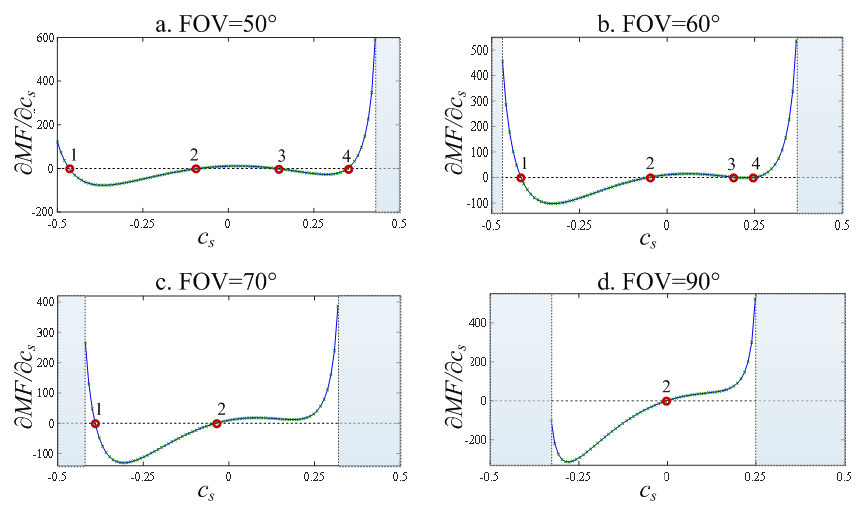
\includegraphics[width=.85\textwidth]{chapter-3/figures/PhaseTransition_field.png}
    \caption{SPC scan curves for different values of the FOV. Shaded areas are ray failure regions. The scan curves are obtained in the same way as the one shown in Figure \ref{fig:SPCscan}. Saddle point curvatures are marked by red circles. With the increase of the FOV, saddle point 1 disappears in the ray failure region. SP3 and SP4 merge with the minimum between them, and are replaced by a saddle point (not shown) that is not constructible with SPC.}
    \label{fig:phasechange_field}
\end{figure}

A different kind of change is also observed. At 50° [Figure \ref{fig:phasechange_field}(a)] four saddle points can be found. However, at larger fields the third and fourth saddle point first move closer [Figure \ref{fig:phasechange_field}(b)], merge and then disappear [Figure \ref{fig:phasechange_field}(c) and (d)]. 

By optimizing from the saddle points, at 50° it is found that the last two saddle points lead on one side of the saddle to the same minimum. While changing the FOV in small steps, it is possible to keep track of the two saddle points and one minimum by keeping the norm of the gradient to zero via minimization. The process is elaborated in Figure \ref{fig:systemdie}. When the FOV increases from 50° to 60°, it is seen that the Euclidean distances between the saddle points and minimum reduce. Hence the critical points are getting closer in the high-dimensional design space. At 70°, it is no longer possible to find saddle points via an SPC scan. However, it is still possible to obtain the merged point by keeping the norm of the gradient to zero at the vicinity of the previous critical points. From Figure \ref{fig:systemdie}, it is seen that the original two saddle points and one minimum merge into one saddle point with a merit function value of 74.92. It is a saddle point without any null elements, hence it cannot be constructed using SPC. This shows how two saddle points and one minimum merge into one saddle point while the FOV increases. 

\begin{figure}[h!]
    \centering
    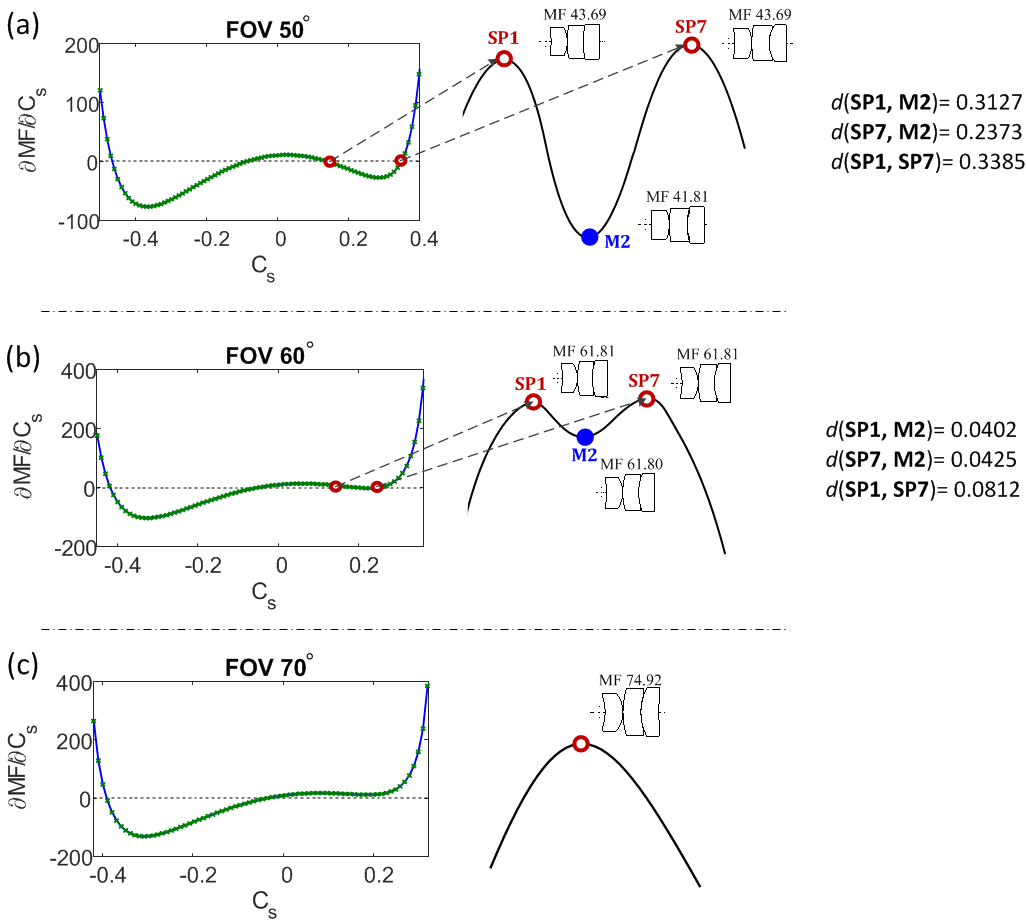
\includegraphics[width=0.8\textwidth]{chapter-3/figures/SystemDie.png}
    \caption{Merging of two saddle points and one minimum when the FOV increases, from Figure (a) to Figure (c). In the SPC scan curves, the two saddle points get closer and then disappear. The two saddle points and one minimum in between merge into one SP. The decreasing Euclidean distances also indicate the merging.}
    \label{fig:systemdie}
\end{figure}

A different phenomenon is observed when FOV increases. In Figure \ref{fig:systemborn}, the two saddle points on the left side of the scan curve are investigated: at 54°, SP8 and SP2 both lead to M9 when optimizing on one side. However, when the FOV increases to 56°, the two saddle points are connected to M3 instead of M9. The minimum M9 is connected to M3 via SP12. M3 and SP12 do not exist when the FOV is 54°. We see that when the FOV increases, a pair of local minimum (M3) and saddle point (SP12) start to emerge. Their merit function values are very close to each other (54.06 vs. 54.07) at 56° FOV. When the FOV increases to 60°, the difference between merit function values increases (61.31 vs. 61.96) as well as the Euclidean distance between M3 and SP12 (increases from 0.1148 to 0.2611). 

Besides merging or splitting, it is also found that in some special situations, when the FOV increases, both approaching and distancing\footnote{When mentioned merging, we observed that a pair of points approach each other and reach a situation where they cannot be distinguished anymore. When mentioned splitting, we observe that one point splits into two and they move away from each other. When this happens in a continuous way with a change of the system setting (e.g. FOV), approaching and distancing is used to describe the behaviour of the two points.} happens for the same pairs. Figure \ref{fig:systemreborn} illustrates a scenario when a glass null element was used as an SPC scan element. The FOV is increased from 60° to 110°, where three steps (60°, 90° and 110°) are plotted in the figure. At 60°, two saddle points were found by the scan. Both of them lead to a common minimum at one side (illustrated on the right of the scan curve). With the increasing of the FOV, the two saddle points become closer in the design landscape: the Euclidean distance reduces from 0.0785 to 0.0023 when the FOV increases from 60° to 90°. At this phase, a much smaller step size of the scan is necessary to be able to find the saddle point. After the FOV increased to 110°, the Euclidean distance between the two increases from 0.0023 to 0.0217. As a result, the tendency of the merging of the two saddle points changes to splitting. 

It is seen in the aforementioned three examples that the change of the design landscape can be dynamic and unpredictable. When a certain design specification changes, it essentially alters the design landscape. This change may affect the number of saddle points and minima which can be obtained with the SPC approach. Nevertheless, for the given examples, redundancy of the saddle point - minimum links also reduces the risk of missing solutions with the SPC approach. All the good solutions were obtained with the SPC method.

\begin{figure}[h!]
    \centering
    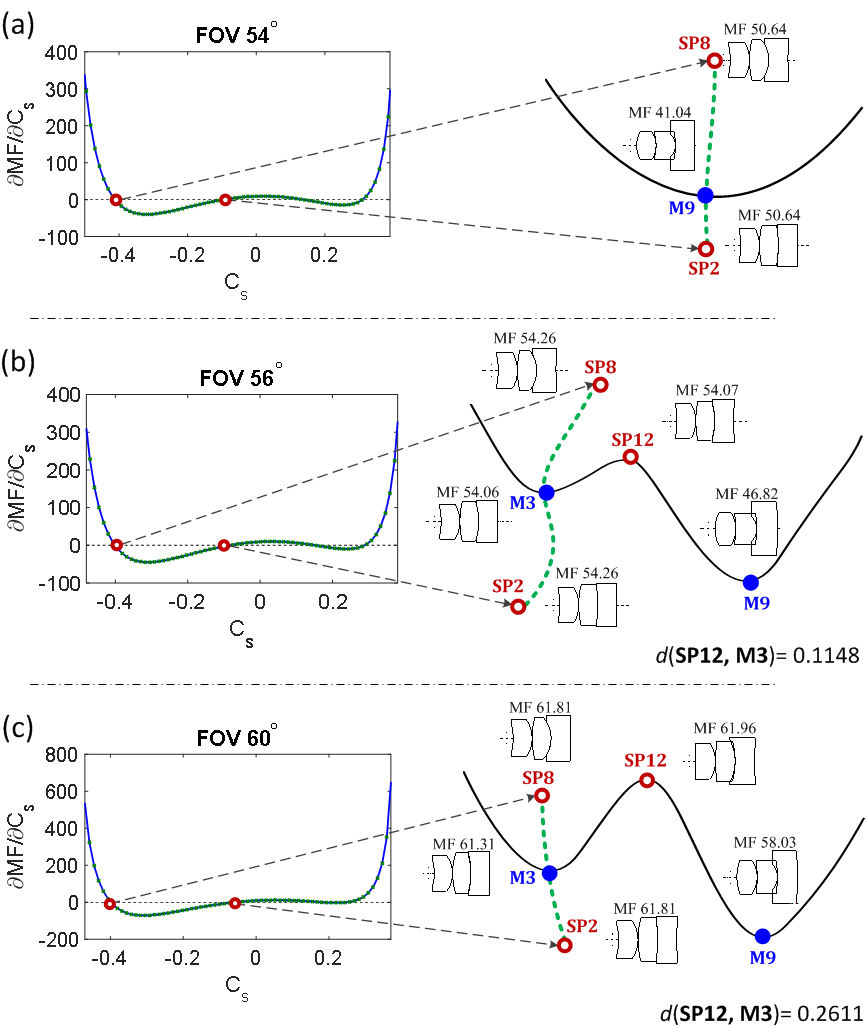
\includegraphics[width=0.75\textwidth]{chapter-3/figures/SystemBorn.png}
    \caption{A pair of minimum - saddle point emerges when FOV increases. From (a) to (c), the FOV increases. M3 and SP12 start to appear and form the link M3-SP12-M9. The connection between saddle points and minima are altered: at 54°, SP8 and SP12 connect to M9; at 56°, SP8 and SP12 connect to M3.}
    \label{fig:systemborn}
\end{figure}

\begin{figure}[h!]
    \centering
    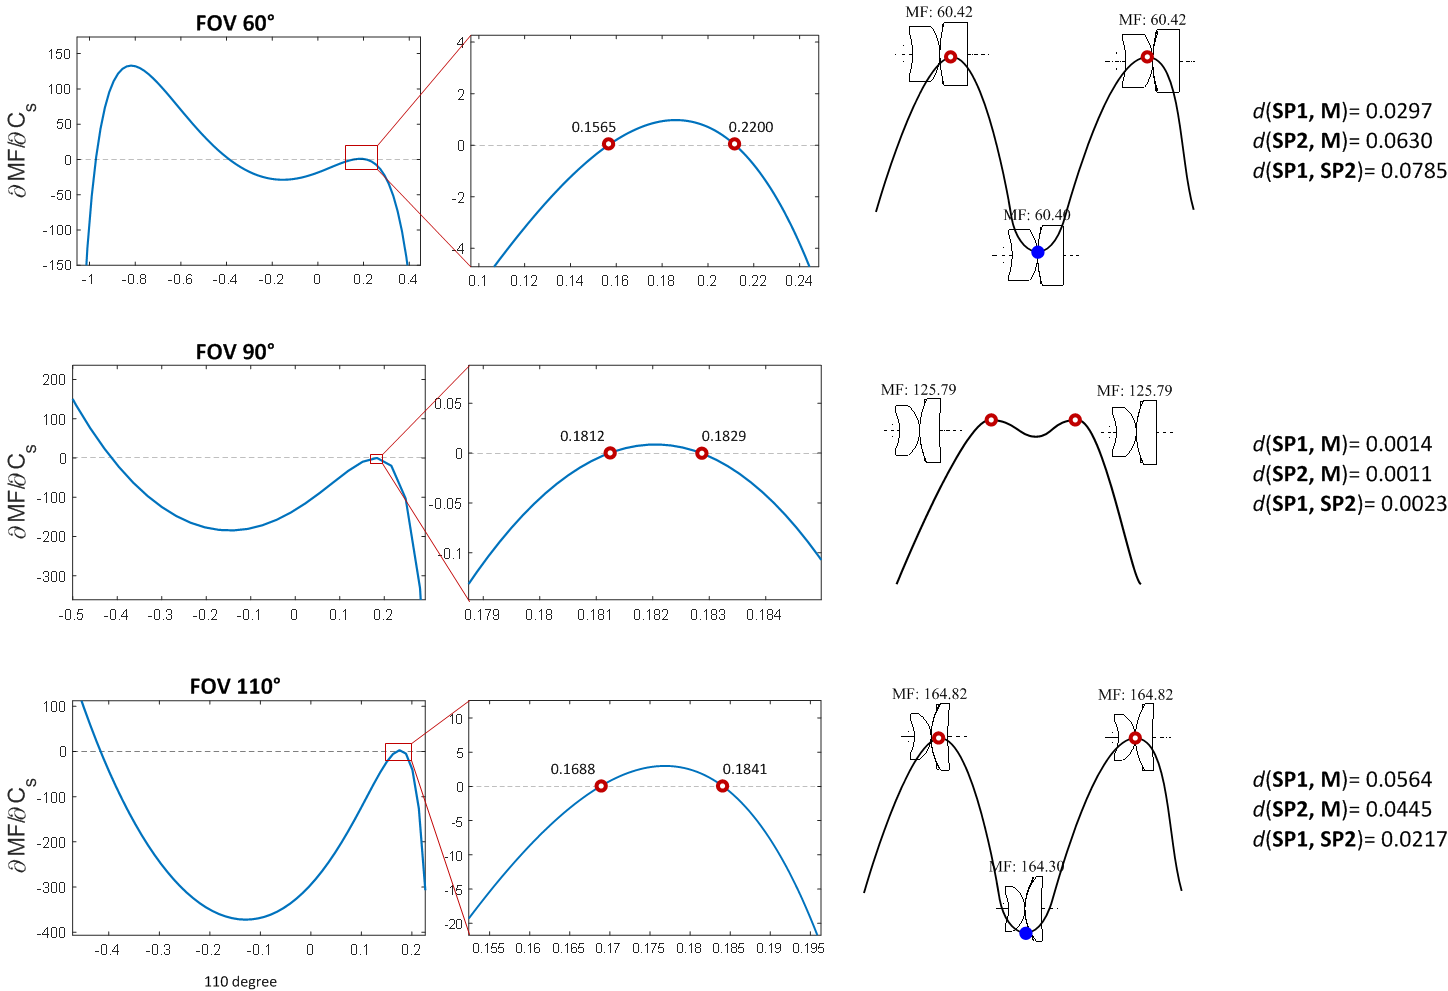
\includegraphics[width=0.8\textwidth]{chapter-3/figures/SystemReborn_vt.png}
    \caption{A glass null-element SPC scan is performed on DB-M1 from Figure \ref{fig:single2double}. The scan position is between the two lens elements. When the FOV increases from 60° to 110°, the two saddle points on the right first get closer, and then further apart. This phenomenon can be observed from the SPC scan curve as well as from the Euclidean distances between the two.}
    \label{fig:systemreborn}
\end{figure}
%%%%%%%%%%%%%%%%%%% Section %%%%%%%%%%%%%%%%%%%%%%%%%%%%%

\section{Discussion and Conclusion}
The design landscape of a wide-angle pinhole lens and its closely related optimization landscape are investigated in this chapter. Several observations that result from this study have a more general validity. Switching between minima with SPC introduced in Subsection \ref{cp2-switching}, is applied to the pinhole lens as shown in Figure \ref{fig:wideangleSwitch}. It can be used in other design tasks as well to avoid the trapping of the optimization in a sub-optimal solution. Combining SPC with conventional design methods, as shown in Figure \ref{fig:WideAngleDesign}, can lead to good complex designs starting from simpler ones \cite{LivshitsSP2014}.

The lens design landscape is different from general global optimization problems because of the close relationship that often exists between the local minima of a design problem and local minima with one lens less. Figure \ref{fig:tripletnetwork} is particularly useful to illustrate this structure, due to the special choices that are made in the corresponding search (lenses in contact, use of air null elements). The systems SP1–SP11 are triplet saddle points, but if the air null-element of the corresponding scan (a pair of surfaces that has no influence at all on the rays or on the merit function) is removed, they become doublet minima. However, when these doublet minima with an extra null-element are optimized on both sides of the resulting saddle, they lead to the triplet minima M1–M10. In the search shown in Figure \ref{fig:tripletnetwork}, these 10 triplet minima are all minima found in the landscape with other methods such as NETMIN and CODE V that are used for comparison. A scenario where this structure holds for all minima has been previously encountered \cite{PascalTriplet2009}. The corresponding landscape is dominated by spherical aberration. The wide angle examples discussed here show that the scenario where this structure is present for most of the minima, can be much more general.

% HZ: the structure is a structure that all minima are connected via saddle points, and these saddle points can be constructed using SPC. Having a trans-dimensional structure of the minima and saddle point does not ensure the connection of the saddle point and minima within the same dimension. Local or global structure?

The example shown in Figure \ref{fig:tripletnetwork} has the advantage that the special structure can be observed in a pure form, where all minima and saddle points are connected and the saddle points can be constructed using SPC. Interference of other features can also be present as seen in the examples: Figure \ref{fig:thicknesschange} indicates that some minima do not have a corresponding system with a zero-thickness element, therefore cannot be obtained following the SPC procedure; Figure \ref{fig:phasechange_field} shows that saddle points which cannot be constructed with SPC are present. In these examples, using SPC cannot always find all minima. Nevertheless, Figure \ref{fig:TripletMonoNetwork} shows an example where even in the presence of the aforementioned features of the landscape, the five solutions with the lowest merit function value found with other methods can still be found with SPC.

The example shown in Figure \ref{fig:phasechange_field} is useful for understanding the transition in the local landscape where saddle points that can be constructed using SPC become ones that cannot be constructed using SPC. In an extreme case where none of the saddle points can be constructed using SPC, the landscape becomes a standard global optimization landscape which does not have the special structure we mentioned. The replacement of the SP3 and SP4 in Figure \ref{fig:phasechange_field} by a saddle point, which cannot be constructed with SPC, shows that the landscape is locally transformed into such a standard global optimization landscape. The process is elaborated in Figure \ref{fig:systemdie}. However, the transition can also happen in the opposite direction if the process (in this case, descreasing the FOV) is reversed: a usual saddle point splits into two saddle points and a minimum in between, and in this case, the two saddle points can be constructed using SPC. This complexity of the design landscape dynamic is further explored in Figure \ref{fig:systemborn} and Figure \ref{fig:systemreborn}: When the FOV is increasing, a pair of minimum - saddle point appears; Two saddle points and a minimum first tend to merge and then tend to separate again. 

Based on the examples shown in this chapter, the complex dynamic of the design landscape can already be observed. However, the structure that enables SPC to obtain good solutions is stable. For systems that are more complex than those presented in this chapter, the utility of SPC will be determined by its practical success, rather than by a detailed study of the entire landscape, which becomes difficult. Systems with bigger complexities are investigated in the next chapter. 

The replacement of high-dimensional searches by several one-dimensional searches plus local optimization can lead to a reduction of the complexity of the search. It can be essential for practical purposes. Compared to global optimization methods where multiple starting points are firstly chosen heuristically and then local optimization is applied, SPC operates in a more systematic way that starting points are provided based on constructed saddle points. In computer programs where the search for new solutions is automated, the general version of SPC could be combined with other methods. In the case of the special version of SPC this has already been achieved in the commercial software SYNOPSYS \cite{DilworthSP2012}. Excepting simple problems, no known global optimization method can guarantee finding all (good) solutions in a reasonable time, and SPC is no exception. However, high-quality designs have already been obtained with the special \cite{MarinescuSP2008}\cite{BociortPatent2010} and with the general versions \cite{LivshitsSP2014} of SPC. SPC will finally be validated if many high-quality designs are obtained with this method.

%We have seen that in lens design we can find good solutions with SPC. This method could also be applicable in other design problems where the conditions described in Sections 3 and 4 of \cite{MVTurnhoutSPC15} or in the Appendix of \cite{BociortToyModel2010} are satisfied. In a different multi-parameter optimization problem, if there is a way to construct a
%saddle point in the design landscape, then in principle, it should be possible to follow the same procedure as in lens design to search for new solutions.


\references{dissertation}



%% Use letters for the chapter numbers of the appendices.
\appendix

%\include{appendix-a/appendix-a}

%% Turn off thumb indices for unnumbered chapters.
\thumbfalse

\chapter*{Summary}
\addcontentsline{toc}{chapter}{Summary}
\setheader{Summary}

In this thesis, we explore how lens design and optimization techniques can adapt to the design (optimization) space in order to increase the lens design efficiency. 

The optical lens design space is known to be very complicated. This is a high-dimensional space defined by the degrees of freedom and the quantified performance of a parameterized optical system. This space is also nonlinear which means there are multiple local minima (you can think of the bottom of a crater in the geological landscape) with different values. In modern optical lens design, the task can be described as searching for the global minimal value in the high-dimensional space. For sophisticated lens designs, the number of the degrees of freedom increases in order to gain more control of the design. It brings two major difficulties:  
\begin{enumerate}[nosep]
\item The size of the high dimensional space increases according to the power law which means a brute force search is practically impossible. 
\item The number of local minima increases with the number of the degrees of freedom used. It indicates the number of undesired local minima becomes larger. Hence, the difficulty of finding best minima also increases.  


\end{enumerate}

% technique has been developed 
Over the past decades, different design and optimization techniques have been examined on their effectiveness of obtaining a global optimal solution. Some of the techniques have been integrated into commercial lens design software. However, these algorithms are based almost exclusively on generally applicable mathematical models and use little or no specific knowledge about the optical system (and its design landscape). As a result, little information is available on how these techniques should be used in a practical design task instead of implementing them as a lottery draw. 

We emphasize in this thesis that, considering an actual lens design process, the design space is not only statically complicated, but also dynamically changes through the design process. The dynamic aspect affects the design landscape. As a consequence, the number of local minima and the effectiveness of the optimization techniques can be impacted. In Chapter \ref{chapter_5_SMS}, a study using Simultaneous Multiple Surface (SMS) method as one of the design strategies, compares the effectiveness of different strategies under static and dynamic design landscape.

Saddle Point Construction (SPC) is a design method which can rapidly construct saddle points with Morse Index 1 in a design space. These saddle points serve as agents to guide the local optimization to obtain new minima. Different from other optimization techniques, it also reveals a special structure in the lens design landscape: certain saddle points existing in the landscape are reducible to minima of simpler systems plus one additional lens element.

Previous research shows potentials of SPC as a systematic lens design technique. In this thesis, we further examine the practicality of SPC as a global optimization and semi-global optimization (to generate a small pool of solutions) tool. The dynamic aspect of the design space is particularly of interest since it is relevant to an actual design practice. 

To assess the robustness of SPC as a global optimization method, we examine the solution network of saddle points and minima for several scenarios. We formulate three falsifiable research questions and have falsified two of them based on the observations:
\begin{enumerate}[nosep]
\item In a lens design landscape, are all the saddle points able to be constructed using SPC? The answer to this question is no. The detail of the analysis is given in Chapter \ref{chapter_SPC_simple_system_landscape}.
\item Are all the minima always linked via the saddle point - minima network revealed by SPC? The answer to this question is also no. The analysis is provided in Chapter \ref{chapter_SPC_simple_system_landscape} and also supported by the wide-angle lens example in Chapter \ref{chapter_4_complex_system_exploration}.
\item Does the saddle points - minima network obtained via SPC always contain the best or the best pool of solutions for lens design? We cannot give an answer to this question. However, in the examples we have examined, the positive side of this question is valid. 
\end{enumerate}

Despite the fact that using SPC does not guarantee capturing all the local minima in the design space, we observe that the good minima are always captured in our examples. Given its systematic way of obtaining local minima, we consider it as a useful global search technique for lens design. 

In addition, in Chapter \ref{chapter_4_complex_system_exploration}, we demonstrate that SPC can be particularly effective for complicated systems when the goal is to get a small pool of solution candidates while the system configuration is not drastically changed. 

\begin{comment}
At last, we provide our thoughts on how the lens design landscape can be further studied. However, it is not straightforward how it can be related to an everyday design task. We believe that a tool gets improved during its practice, therefore, suggestions on further making SPC as a practical lens design tool are also given at the end. 
\end{comment}


\begin{comment}
We analyze the characteristics of the optical lens design space. We emphasize its dynamic property, which means the landscape changes given different design condition is changed, which is a common thing during the design practice

This dissertation addresses the typical problem during optical design or generally all engineering problem -- how to find the best solutions in a parameterized system. 

Goal/Nature of the problem: find the best solution -> assess whether the solution is sufficient or not, if it is not, the process should go to the next design decision; if it is sufficient, the solution can be taken. 

How: Parameterize the system with the multiple variables with a model representing its physical property therefore the performance can be evaluated.  
Given the model, use mathematical tools to optimize in order to get the best solution.
(alternatively, you can realize this by continuous testing and modifying during your manufacture -> caveman's method)

  Sub-problem statement: after parameterization, the optimization space of the system is usually a non-convex space, which indicates a presence of multiple local minima when a typical local optimizer is used. Situation of non-convex space provides difficulties in getting a satisfactory solution: it is difficult to find all the existing solutions in the design space. With incomplete set of information, the following question exist: will there be a better solution if one keeps searching given the current system configuration. As a results, techniques that can quickly generate new solutions given a design configuration is welcome to verify if a better system can be found. The process usually ends when a good enough result is found or a time limit is reached. 

Goal: Find whether there is a better solution in a non-convex optimization problem. This is global optimization. 

How: 
1) starting from a very good starting point (this indicates good technique is needed to construct the starting points) and after arriving at a local minimum, GO technique is used to check whether better solutions can be found (the anticipation is not). 

2) starting from somewhat working point (this indicates small effort to determine the starting point) and combined with GO technique to see if we could find more better solutions. The anticipation is that there would be some better results appear. 

    Sub-problem statement: SPC is a GO technique. SPC shows systematic approach and reveals certain structure between optimization landscape and the optical design model. The following questions are interesting regarding SPC:
1) How SPC is performing as a GO technique? In terms of the completeness and efficiency for finding new solutions. Completeness -> do I find every solution, or at least all solutions find by other algorithms.  Efficiency-> what is the time needed to run such GO. Is it a limited amount of algorithmic trial?
2) Does it show more profound connection to the lens design problem such that it could be used to facilitate the design more? This question should be implicitly included in the first one. It is more of scientific curiosity that if the nature of SPC is connected to the lens design problem. 

    Sub-problem statement: SMS is a starting-point-generating technique. The hypothesis is that it generates a good starting point since the method is guided by the physical rules (Fermat's Principle). Is SMS method the method that providing the starting point that close to the best local minimum (via one local optimizer)? 
    
To sum, it is the balance between the effort of getting a good starting point and running less optimization. SPC as an optimization technique needed to be investigated for its GO efficiency. It means, given a non-perfect starting point, the GO method is preferred to efficiently find the best solution. Chapter 2-4 is trying to clarify this.
SMS as a technique to construct starting points, the ultimate question is that if it constructs the starting point that the minimum optimization effort it needed. Chapter 5 is trying to answer this question. 
\end{comment}
\chapter*{Samenvatting}
\addcontentsline{toc}{chapter}{Samenvatting}
\setheader{Samenvatting}

{\selectlanguage{dutch}

Samenvatting in het Nederlands\ldots

\noindent geschreven worden ...

}


\chapter*{Curriculum Vit\ae}
\addcontentsline{toc}{chapter}{Curriculum Vit\ae}
\setheader{Curriculum Vit\ae}

%% Print the full name of the author.
\makeatletter
\authors{\@firstname\ {\titleshape\@lastname}}
\makeatother

\noindent
\begin{tabular}{p{4\parindent}l}
    20-03-1988 & Born in Nei Mongol, P. R. China 
\end{tabular}

\section*{Work Experience}
\begin{tabular}{p{4\parindent}l}
    2019--Now & YieldStar Application, ASML (Eindhoven, the Netherlands) \\

    \\
\end{tabular}

\section*{Education}
\begin{tabular}{p{4\parindent}l}

    2013--2018 & PhD Candidate \\
    & Delft University of Technology (Delft, the Netherlands)\\
    & Datalogic (Bologna, Italy, Jan--May, 2016)\\
    & Polytechnic University of Madrid (Madrid, Oct--Dec, 2015)\\
    \\
    2011-2013 & Master Applied Physics \\
    & Erasmus Mundus OpSciTech (Optical Science and Technology)\\
    &Delft University of Technology (Delft, the Netherlands, 2012--2013)\\
    &Warsaw University of Technology (Warsaw, Poland, 2011--2012)\\
    \\
    2007--2011 & Bachelor Optical Engineering\\
    & Zhejiang University (Hangzhou, P. R. China)
    
\end{tabular}
    
\begin{comment}
\begin{tabular}
    %% The width of the second column is the width of the page, minus the width
    %% of the first column (4\parindent) minus four times the separation between
    %% the start of the column and its contents.
    \begin{minipage}{\textwidth-4\parindent-4\tabcolsep}
        %% We divide the minipage 20/80.
        \begin{tabular}{@{}p{0.2\linewidth}@{}p{0.8\linewidth-\tabcolsep}}
            \textit{Thesis:} & Eine neue Bestimmung der Molek\"uldimensionen \\
            \textit{Promotor:} & Prof.\ dr.\ A.\ Kleiner
        \end{tabular}
    \end{minipage}
\end{tabular}
\end{comment}
\begin{comment}
\section*{Awards}

\begin{tabular}{p{4\parindent}l}
    1922 & Nobel Prize in Physics \\
    \\
    1925 & Copley Medal \\
    \\
    1929 & Max Planck Medal \\
    \\
    1999 & Time magazine's person of the century
\end{tabular}
\end{comment}

\chapter*{List of Publications}
\addcontentsline{toc}{chapter}{List of Publications}
\setheader{List of Publications}
\label{publications}

%% We use the 'etaremune' environment (the reverse of 'enumerate') to get a
%% numbered list of publications in reverse chronological order. If the list of
%% authors is long, it might be useful to emphasize your own name with \textbf.
\Large{\textbf{Refereed publications}}

\begin{enumerate}\small{
\item \textbf{Z.\ Hou},  M. Nikolic, P. Benitez, and F. Bociort, "SMS2D designs as starting points for lens optimization," \href{https://doi.org/10.1364/OE.26.032463}{\textit{Opt. Express} \textbf{26}, 32463-32474 (2018)}.
\item \textbf{Z.\ Hou}, I. Livshits, and F. Bociort, "One-dimensional searches for finding new lens design solutions efficiently," \href{https://doi.org/10.1364/AO.55.010449}{\textit{Appl. Opt.} \textbf{55}, 10449-10456 (2016)}. 
\item A. Reyes-Reyes, \textbf{Z.\ Hou}, E. van Mastrigt, R. C. Horsten, J. C. de Jongste, M. W. Pijnenburg, H. P. Urbach, and N. Bhattacharya, "Multicomponent gas analysis using broadband quantum cascade laser spectroscopy," \href{https://doi.org/10.1364/OE.22.018299}{\textit{Opt. Express} \textbf{22}, 18299-18309 (2014)}.
}\end{enumerate}

\vspace{3mm}
\noindent
\Large{\textbf{Conference proceedings}}
\begin{enumerate}\small{
\item \textbf{Z.\ Hou},  I. Livshits, and F. Bociort, "Practical use of saddle-point construction in lens design," \href{https://doi.org/10.1117/12.2312494}{\textit{Proc. SPIE} \textbf{10690}, Optical Design and Engineering VII, 1069007 (2018)}.
\item \textbf{Z.\ Hou} and F. Bociort, "Reducible complexity in lens design," \href{https://doi.org/10.1117/12.2191364}{\textit{Proc. SPIE} \textbf{9626}, Optical Systems Design 2015: Optical Design and Engineering VI, 96260J (2015)}.
\item I. Livshits, \textbf{Z. Hou}, P. van Grol, Y. Shao, M. van Turnhout, P. Urbach, and F. Bociort, "Using saddle points for challenging optical design tasks," \href{https://doi.org/10.1117/12.2061975}{\textit{Proc. SPIE} \textbf{9192}, Current Developments in Lens Design and Optical Engineering XV, 919204 (2014)}.

}\end{enumerate}

\vspace{3mm}
\noindent
\Large{\textbf{Conference contributions}}
\begin{enumerate}\small{
\item \textbf{Z. Hou}, Y. Zhang, and F. Bociort, "Design Using Saddle Point Construction in Complex Lens Systems," oral presentation at the European Optical Society Biennial Meeting, Delft, the Netherlands (October 2018).
\item \textbf{Z. Hou}, I. Livshits, and F. Bociort, "Practical use of saddle-point construction in lens design," oral presentation at the SPIE Optical Systems Design conference, Frankfurt, Germany (May 2018).
\item \textbf{Z. Hou}, "One-dimensional searches for finding new lens design solutions efficiently,"  Excellent Oral Presentation Award at the International Doctoral Students Conference on "Opportunities and Challenges Arises from Global Technological Revolution", Zhejiang, China (May 2017).
\item \textbf{Z. Hou}, F. Bociort, I. Livshits, and H.P. Urbach, "A systematic study on the design landscape of a pin-hole lens," oral presentation at the 10th International Conference on Optics-photonics Design and Fabrication, Weingarten, Germany  (March 2016).
\item \textbf{Z. Hou}, F. Bociort, and I. Livshits, "Reducible complexity in lens design - 
replacing high-dimensional search by one-dimensional searches to find new solutions efficiently," poster presentation at the IST Science Day, Delft, the Netherlands (October 2015).
\textbf{Z. Hou} and F. Bociort, "Reducible complexity in lens design," invited Paper at the SPIE Optical Systems Design conference, Jena, Germany (September 2015). 
\item F. Bociort, P. van Grol, I. Livshits, \textbf{Z. Hou}, Y. Shao, P. Urbach, "Saddle-point methods for systematic design," the European Optical Society Biennial Meeting, Berlin Adlershof, Germany (September 2014).
I. Livshits, \textbf{Z. Hou}, P. van Grol, Y. Shao, M. van Turnhout, P. Urbach, and F. Bociort, "Using saddle points for challenging optical design tasks," the SPIE OPTICAL ENGINEERING + APPLICATIONS conference, San Diego, U.S.A. (August 2014).

}\end{enumerate}


\end{document}

